\documentclass[pdflatex, ngerman]{beamer}
%~ \setbeameroption{show notes}

\usepackage[T1]{fontenc}
\usepackage[utf8]{inputenc}
\usepackage[ngerman]{babel}
%~ \usepackage[babel]{csquotes}
%~ \usepackage{cite}
\usepackage{hyperref}
%~ \usepackage{color}
%~ \usepackage{listings}
%~ \usepackage{amsmath,amsfonts,amssymb}
\usepackage{graphicx}
\graphicspath{{./images/}}

\usepackage{multirow}

%~ because tikz rocks
%~ \usepackage{tikz}
%~ \usetikzlibrary{calc,decorations.pathmorphing,patterns}

\usepackage{MyriadPro}
\usepackage{MinionPro}

%~ \usetheme{Amsterdam}
\DeclareOptionBeamer{compress}{\beamer@compresstrue}
\ProcessOptionsBeamer

\mode<presentation>

\useoutertheme{infolines}
\useinnertheme{rectangles}
\usecolortheme{whale}
\usecolortheme{orchid}

\definecolor{beamer@blendedblue}{rgb}{0.137,0.466,0.741}

\setbeamercolor{structure}{fg=beamer@blendedblue}
\setbeamercolor{titlelike}{parent=structure}
\setbeamercolor{frametitle}{fg=black}
\setbeamercolor{title}{fg=black}
\setbeamercolor{item}{fg=black}

\beamertemplatenavigationsymbolsempty

\let\oldnote\note
\renewcommand{\note}[1]{\oldnote{#1\par}}
\newcommand{\mynote}[2]{{\note{\textbf{#1} #2}}}
\newcommand{\demo}{%
\begingroup
	\setbeamercolor{background canvas}{bg=black}
	\begin{frame}[plain]
	\end{frame}
\endgroup
}

\title[Server NAS]{Server -- NAS}
\subtitle[Kurzform]{Private Sicherheitskopien vor Erdbeben, \\ kosmischer Hintergrundstrahlung und dem BKA schützen}
\author[Moritz Schlarb]{Moritz Schlarb}
\institute[JGU Mainz]{Institut für Informatik\\ Johannes Gutenberg-Universität Mainz}
\date[08.01.2013]{08. Januar 2013}
\subject{Learn Linux the Hard Way}
\keywords{RAID, LVM, LUKS, CIFS, Samba, NFS, rsync}

\titlegraphic{
\includegraphics[scale=0.1]{logo}}

\setcounter{tocdepth}{2}
\begin{document}

\frame{
	\titlepage
}

\frame{
	\frametitle{Inhaltsverzeichnis}
	\tableofcontents
}

\begin{frame}{Easy vs. Awesome}
\begin{columns}
\column{.45\textwidth}
\begin{block}{\textbf{Easy:} \\ D-Link DNS-320}<1->
\centering 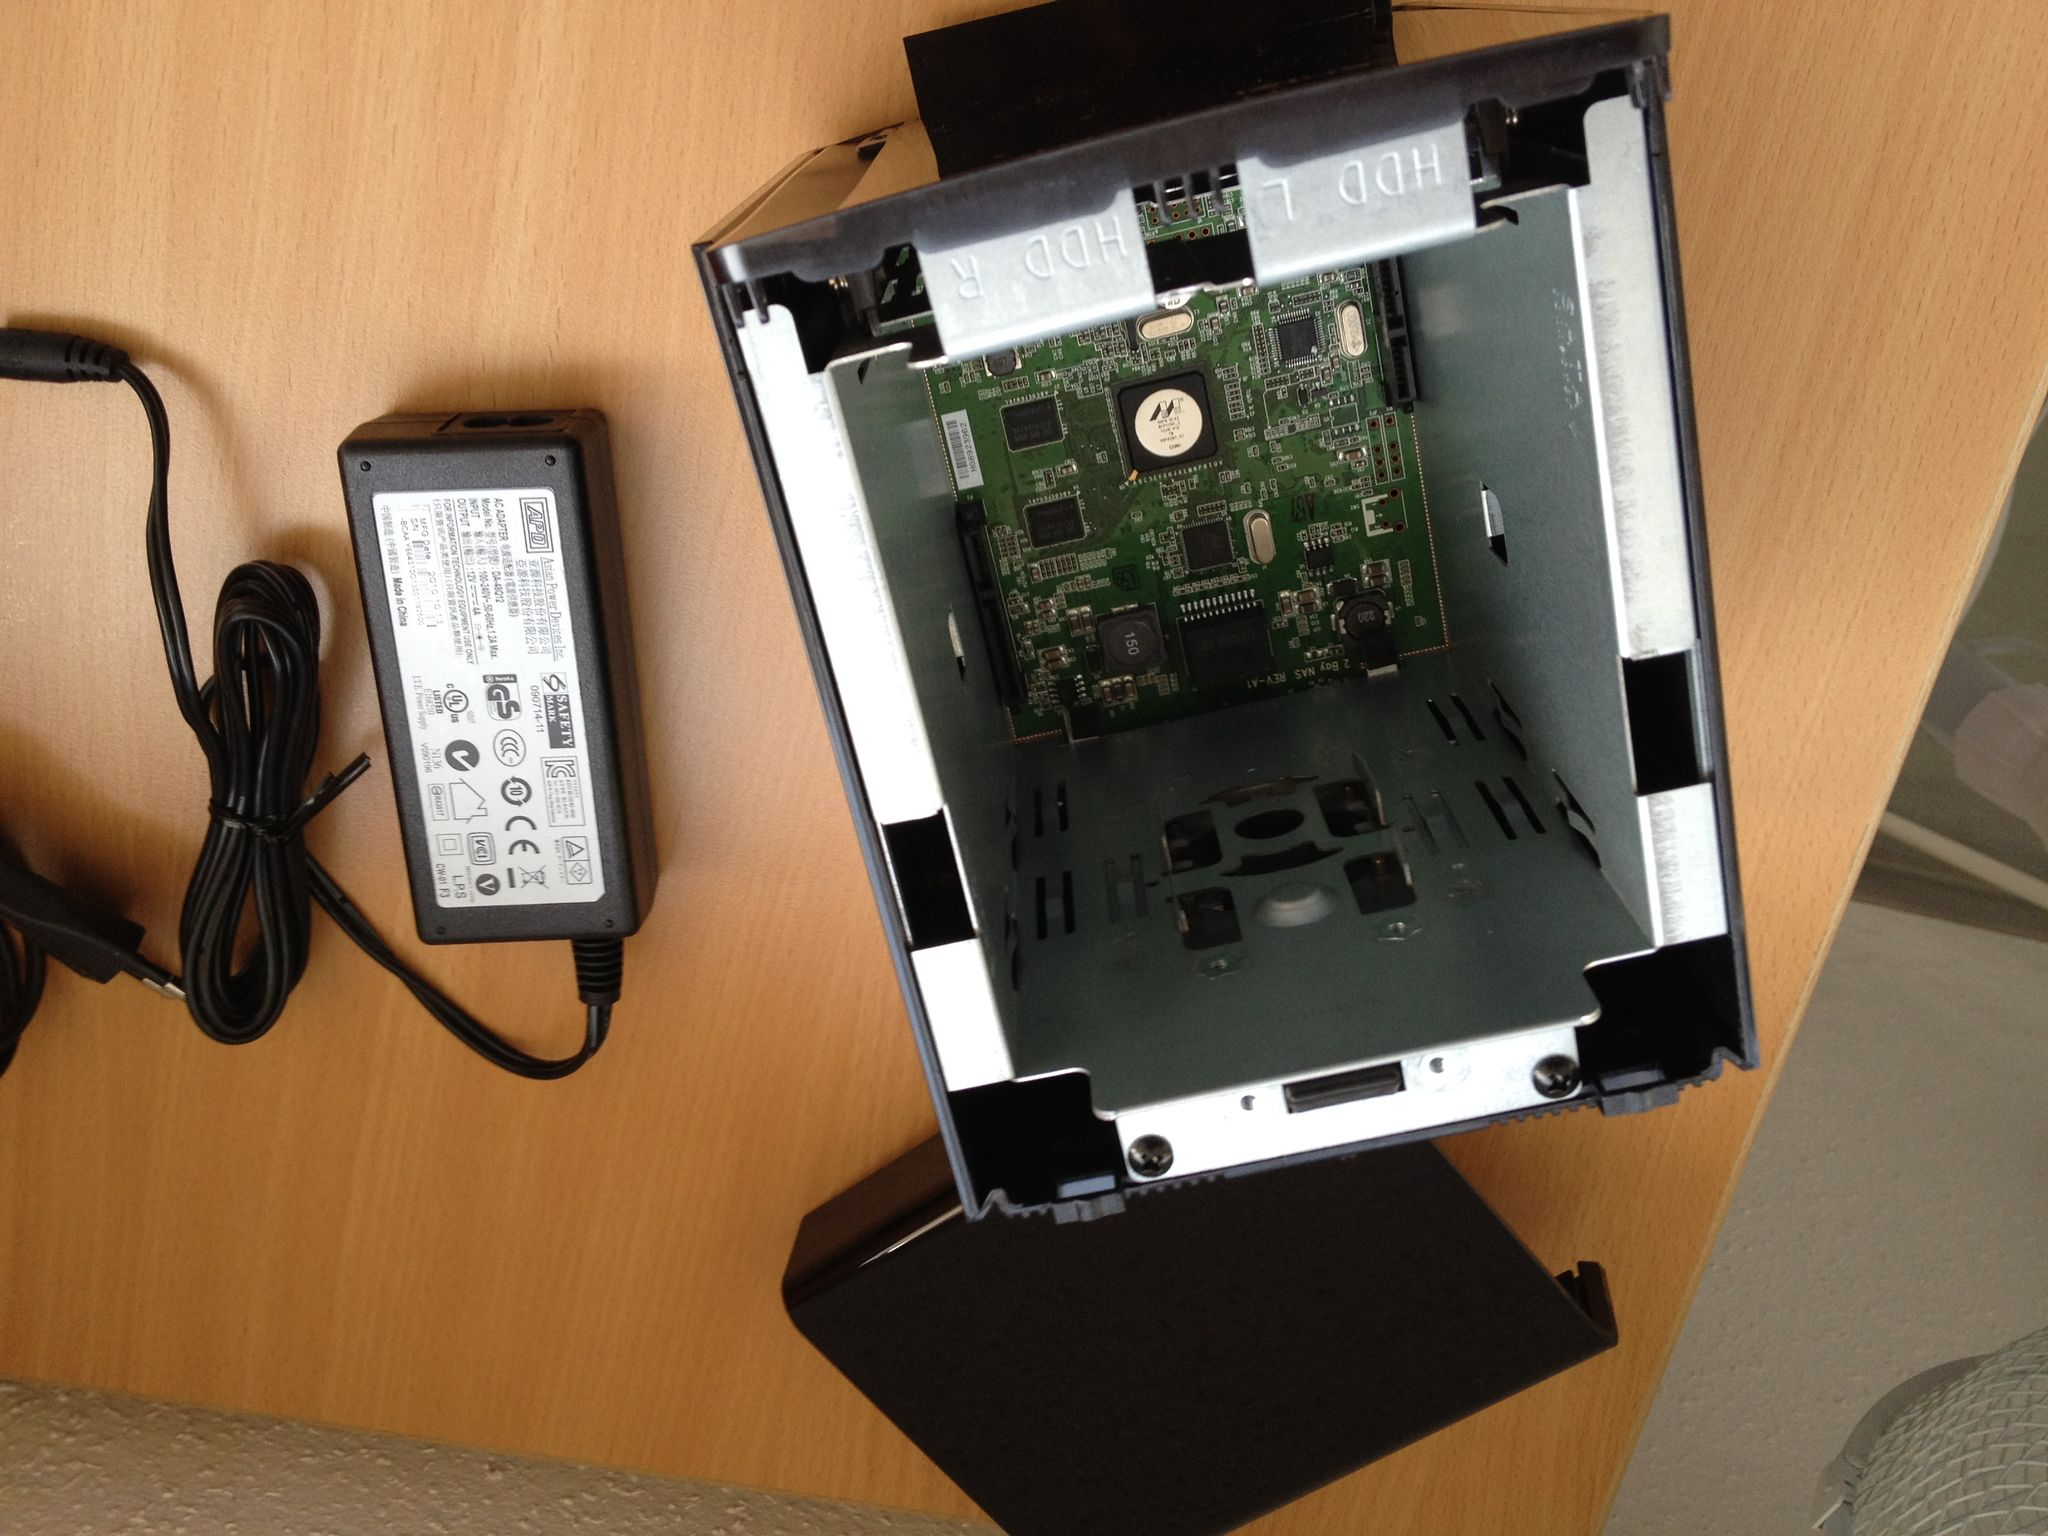
\includegraphics[width=0.9\columnwidth,angle=180]{dns320_.jpg}
\begin{footnotesize}
  \begin{itemize}
    \item \textbf{CPU:} Marvell 88F6281, \\ 800MHz, ARMv5
    \item \textbf{RAM:} 128 MB
    \item \textbf{SATA:} 2x SATA II
    \item \textbf{OS:} Firmware (Embedded Linux)
  \end{itemize}
\end{footnotesize}
\end{block}
\mynote{DNS320:}{70 €}
\column{.45\textwidth}
\begin{block}{\textbf{Awesome:} \\ HP Proliant Microserver N40L}<2->
\centering 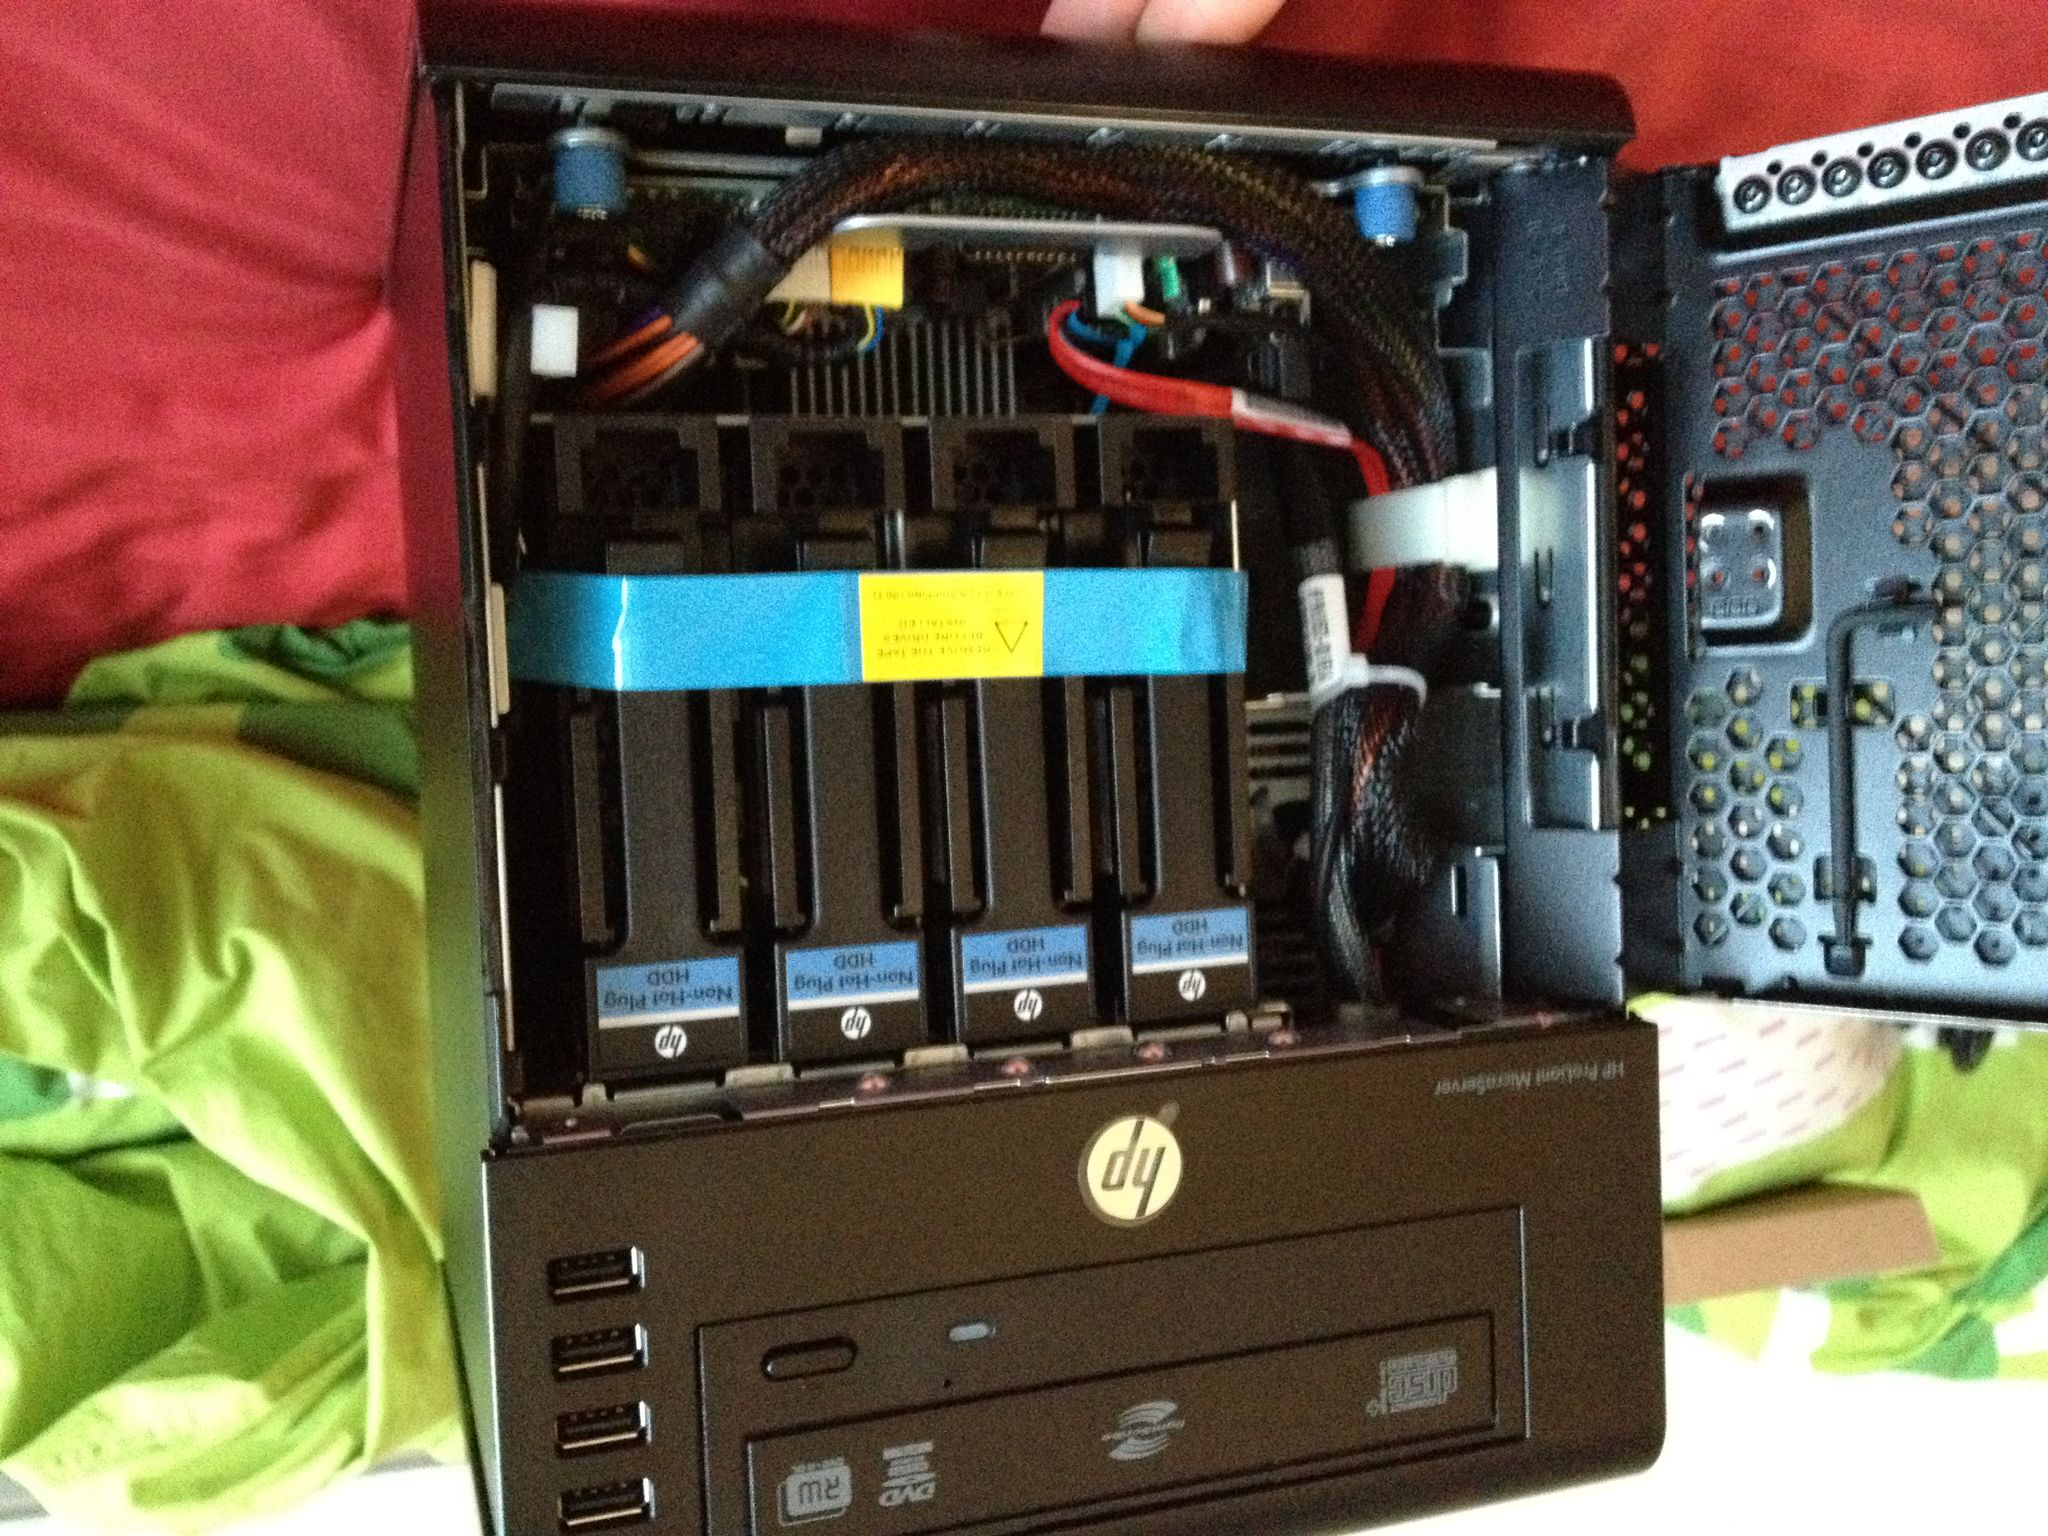
\includegraphics[width=0.9\columnwidth,angle=180]{n40l_.jpg}
\begin{footnotesize}
  \begin{itemize}
    \item \textbf{CPU:} {AMD Turion II Neo N40L}, \\ 2x 1,5 GHz, AMD64
    \item \textbf{RAM:} 2 -- 16 GB
    \item \textbf{SATA:} 5x SATA II
    \item \textbf{OS:} n/a
  \end{itemize}
\end{footnotesize}
\end{block}
\mynote{N40L:}{200 €}
\end{columns}
\end{frame}

\section{Virtualisierung mit Bordmitteln}

\subsection{KVM}

\begin{frame}{QEMU}
\centering
\includegraphics[width=0.2\columnwidth]{qemu-logo}

\begin{block}{}
  \begin{itemize}
    \item ``Quick Emulator'' \mynote{Quick:}{not}
    \item Kann verschiedene Prozessorarchitekturen emulieren: \\
		i386, x86\_64, arm, mips, ppc, \ldots{} \note{\texttt{\$ emerge -pv qemu}\\ \texttt{\$ equery u qemu}}
    \item Emulator für Geräte (Festplatten, Netzwerk-, Sound- und Grafikkarten)
  \end{itemize}
\end{block}
\end{frame}

\begin{frame}{KVM}{Kernel-based Virtual Machine}
\centering
\includegraphics[width=0.5\columnwidth]{kvmbanner-logo2}

\begin{block}{}
  \begin{itemize}
    \item Hypervisor
		\mynote{Hypervisoren:}{Typ 1 (vSphere, Hyper-V, Xen) vs. Typ 2 (VirtualBox, VMWare Workstation)}
    \item Benötigt Prozessor-Unterstützung für Hardware-Virtualisierung: \\
    	Intel (Intel VT) oder AMD (AMD-V) \\
        \texttt{\$ egrep 'vmx|svm' /proc/cpuinfo}
        \mynote{KVM:}{Host-Kernel\\ \texttt{\scriptsize%
-\--\-- Virtualization \\
<*> \- \- Kernel-based Virtual Machine (KVM) support\\
<*> \- \- \- \- KVM for Intel processors support\\
< > \- \- \- \- KVM for AMD processors support\\
}
\texttt{TUN}, \texttt{BRIDGE}, \texttt{VHOST\_NET}
}
    \item Paravirtualisierung durch Virtio
		\mynote{Virtio:}{Guest-Kernel\\ \texttt{\scriptsize%
\$ grep VIRTIO /usr/src/linux/.config \\
CONFIG\_VIRTIO\_BLK=y\\
%~ CONFIG\_SCSI\_VIRTIO=y\\
CONFIG\_VIRTIO\_NET=y\\
%~ CONFIG\_VIRTIO\_CONSOLE=y\\
%~ CONFIG\_HW\_RANDOM\_VIRTIO=y\\
CONFIG\_VIRTIO=y\\
%~ CONFIG\_VIRTIO\_RING=y\\
%~ CONFIG\_VIRTIO\_PCI=y\\
CONFIG\_VIRTIO\_BALLOON=y\\
%~ CONFIG\_VIRTIO\_MMIO=y\\
}}
		\mynote{Paravirtualisierung:}{Softwareschnittstelle ähnlich aber nicht identisch zu echter Hardware, erfordert Portierung des Gastbetriebssystems, Vereinfacht Aufbau der VM und ermöglicht VM mehr Leistung}
  \end{itemize}
\end{block}
\end{frame}

\subsection{libvirt}

\begin{frame}{libvirt}
\centering
\includegraphics[width=0.5\columnwidth]{Libvirt_logo}

\begin{columns}
\column{\textwidth}
\begin{block}{}
  \begin{itemize}
	\item Bibliothek/API/Daemon zur Konfiguration/Steuerung von verschiedenen Virtualisierungsumgebungen
  \end{itemize}
\note{\texttt{\$ emerge -pv libvirt}\\ \texttt{\$ equery u libvirt}}
\end{block}
\end{columns}
\end{frame}

\subsection{virt-manager}

\begin{frame}{virt-manager}
\centering
\includegraphics[width=0.5\columnwidth]{virt-manager_logo}
\begin{block}{}
  \begin{itemize}
    \item Grafisches Frontend für libvirt
    \item Remote-Zugriff auf verschiedene libvirt-Instanzen
  \end{itemize}
\note{\texttt{\$ emerge -pv virt-manager}\\ \texttt{\$ equery u virt-manager}}
\note{virt-manager GUI}
\end{block}
\end{frame}

\demo{}

\section{Partitionierung like a Boss}

\subsection{RAID}

\begin{frame}{RAID}{Redundant Array of Independent/Inexpensive Disks}
\begin{block}{RAID}
\begin{itemize}
	\item Hardware-RAID
	\item Host-RAID
	\item Software-RAID
\end{itemize}
\end{block}
\end{frame}

\begin{frame}{RAID}%{Redundant Array of Independent/Inexpensive Disks}
\begin{columns}
\column{.33\textwidth}<1->
\centering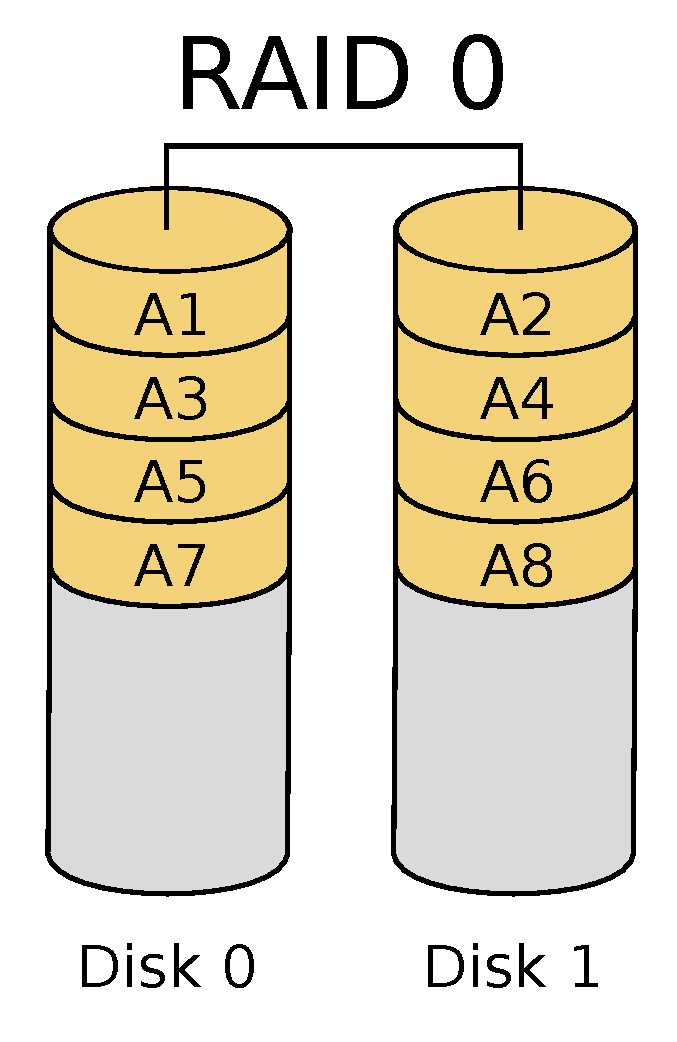
\includegraphics[width=0.9\columnwidth]{/RAID_0}
\column{.33\textwidth}<2->
\centering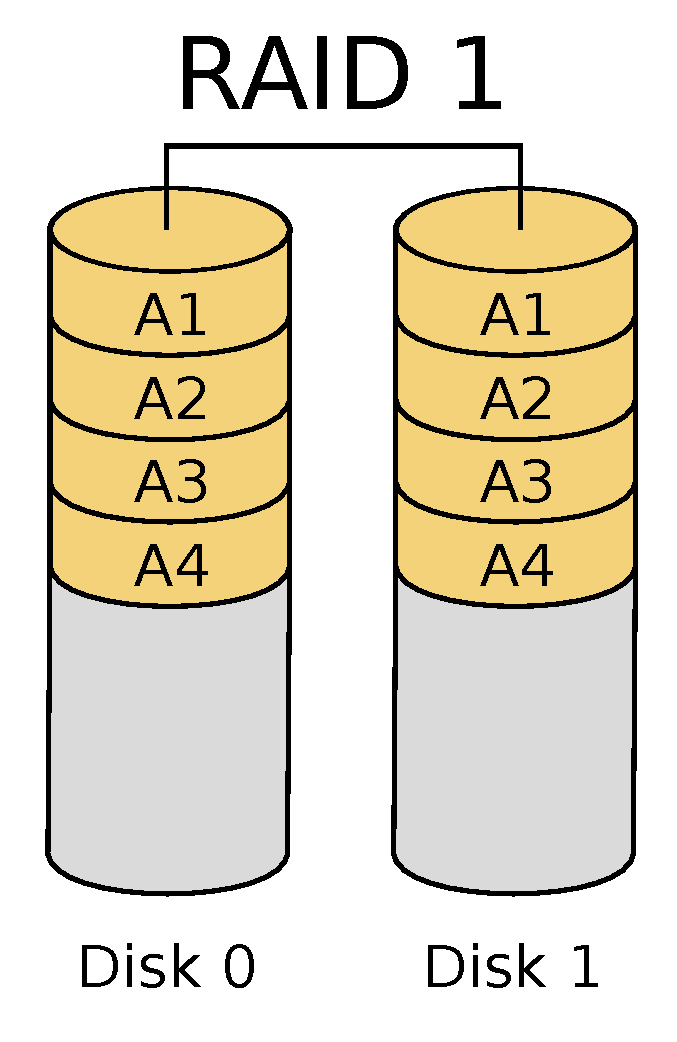
\includegraphics[width=0.9\columnwidth]{/RAID_1}
\end{columns}
\end{frame}

\begin{frame}{RAID}%{Redundant Array of Independent/Inexpensive Disks}
\begin{columns}
\column{.33\textwidth}<1->
\centering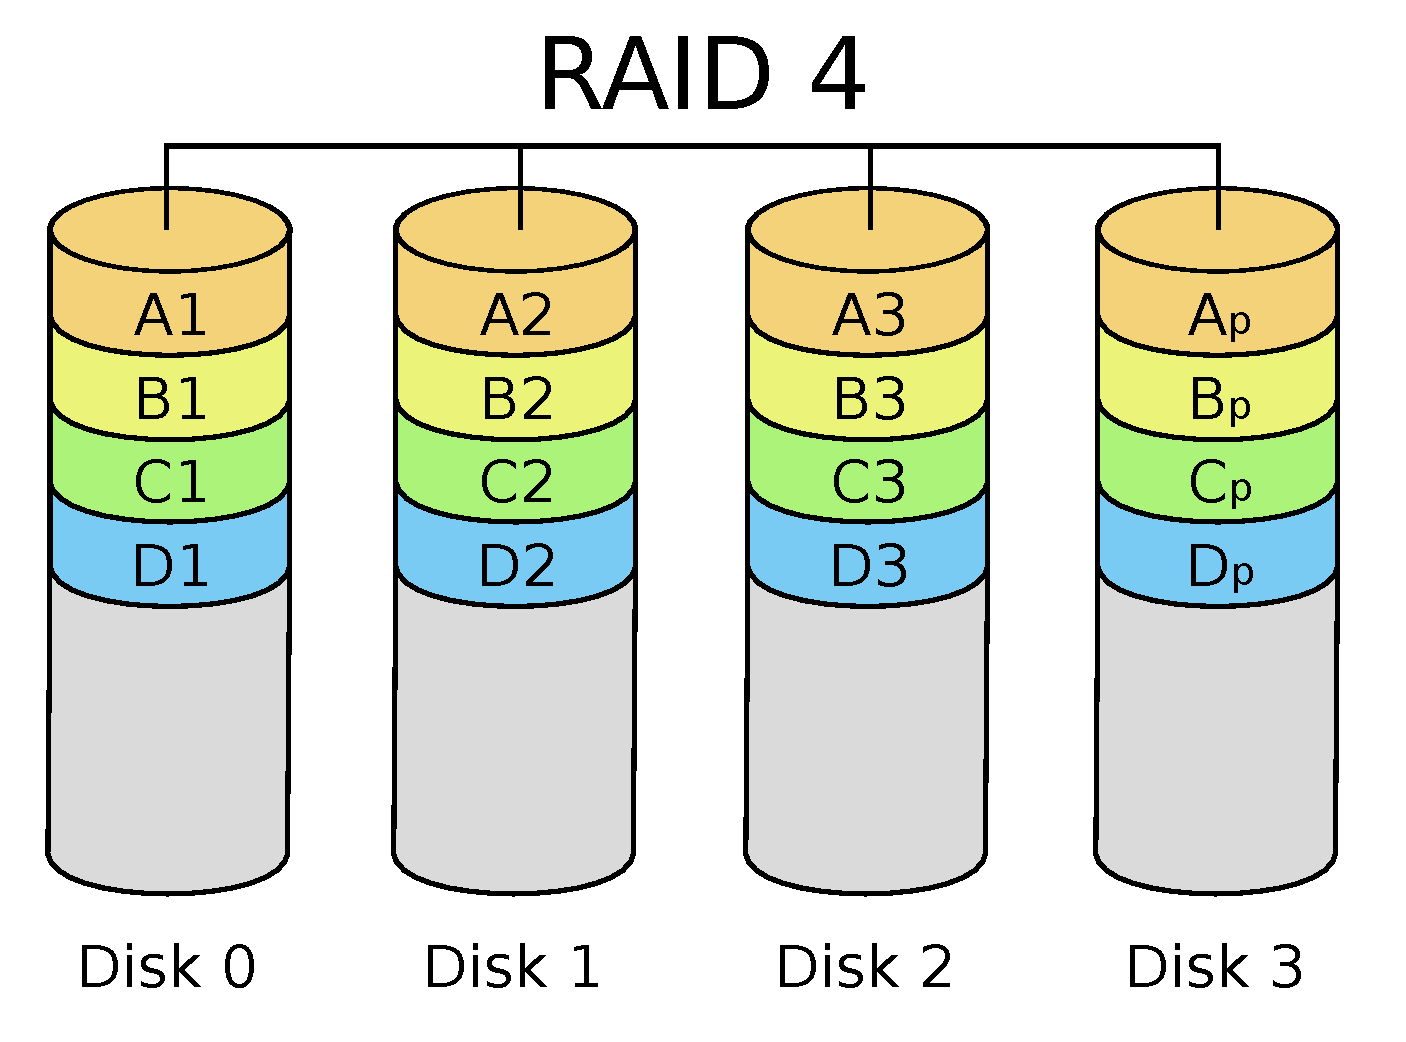
\includegraphics[width=0.9\columnwidth]{/RAID_4}
\column{.33\textwidth}<2->
\centering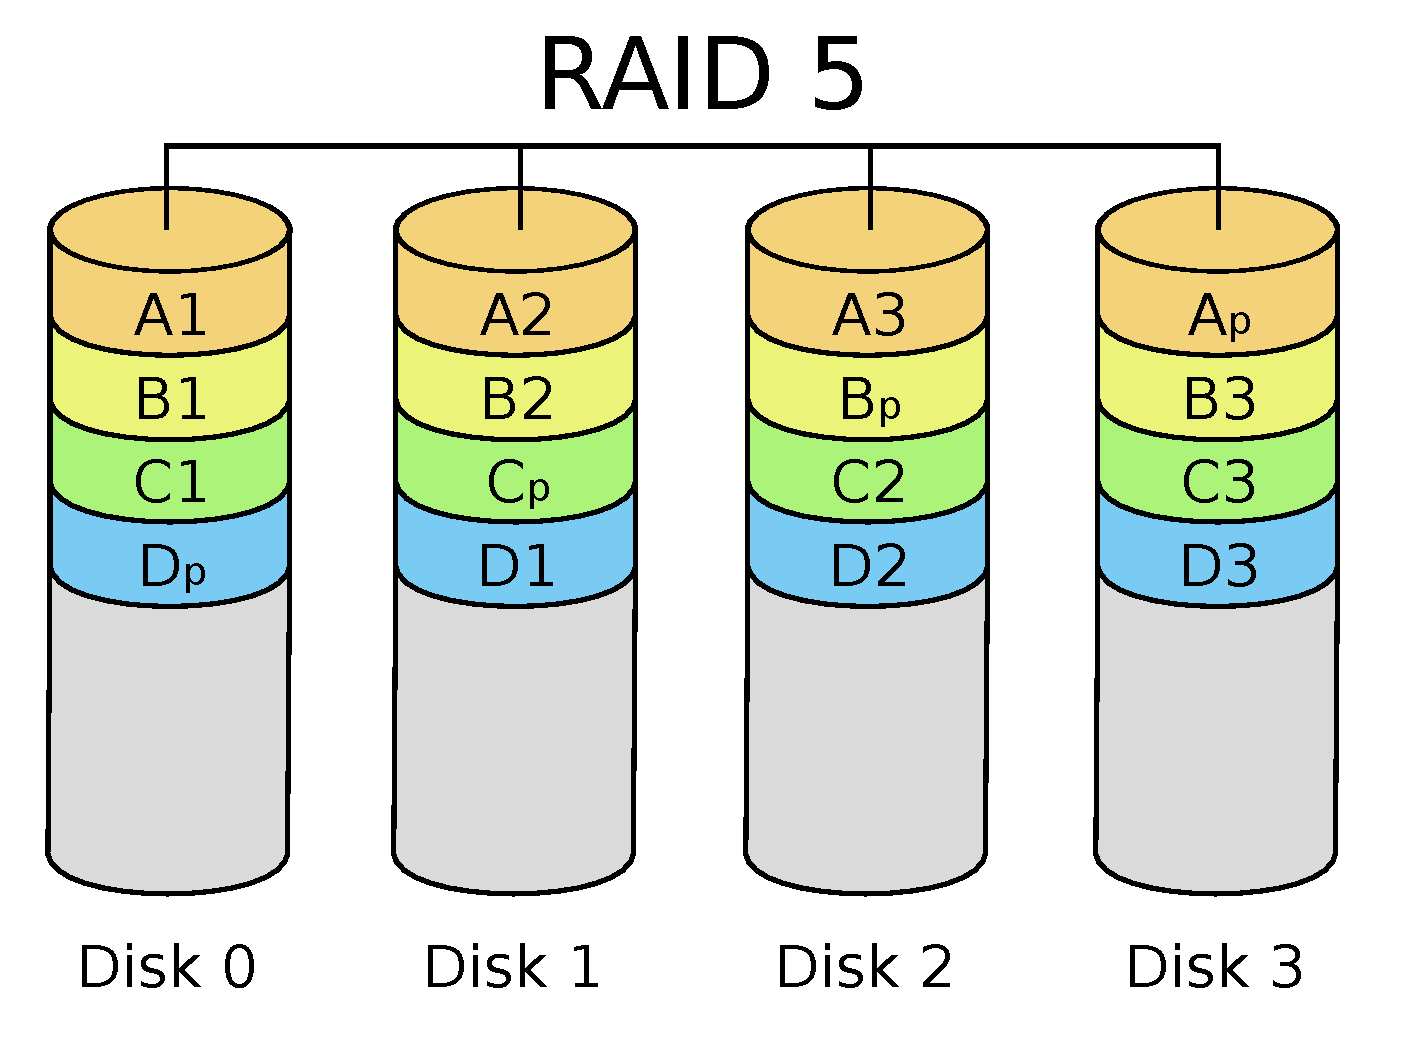
\includegraphics[width=0.9\columnwidth]{/RAID_5}
\end{columns}
\begin{columns}
\column{.5\textwidth}<3->
\centering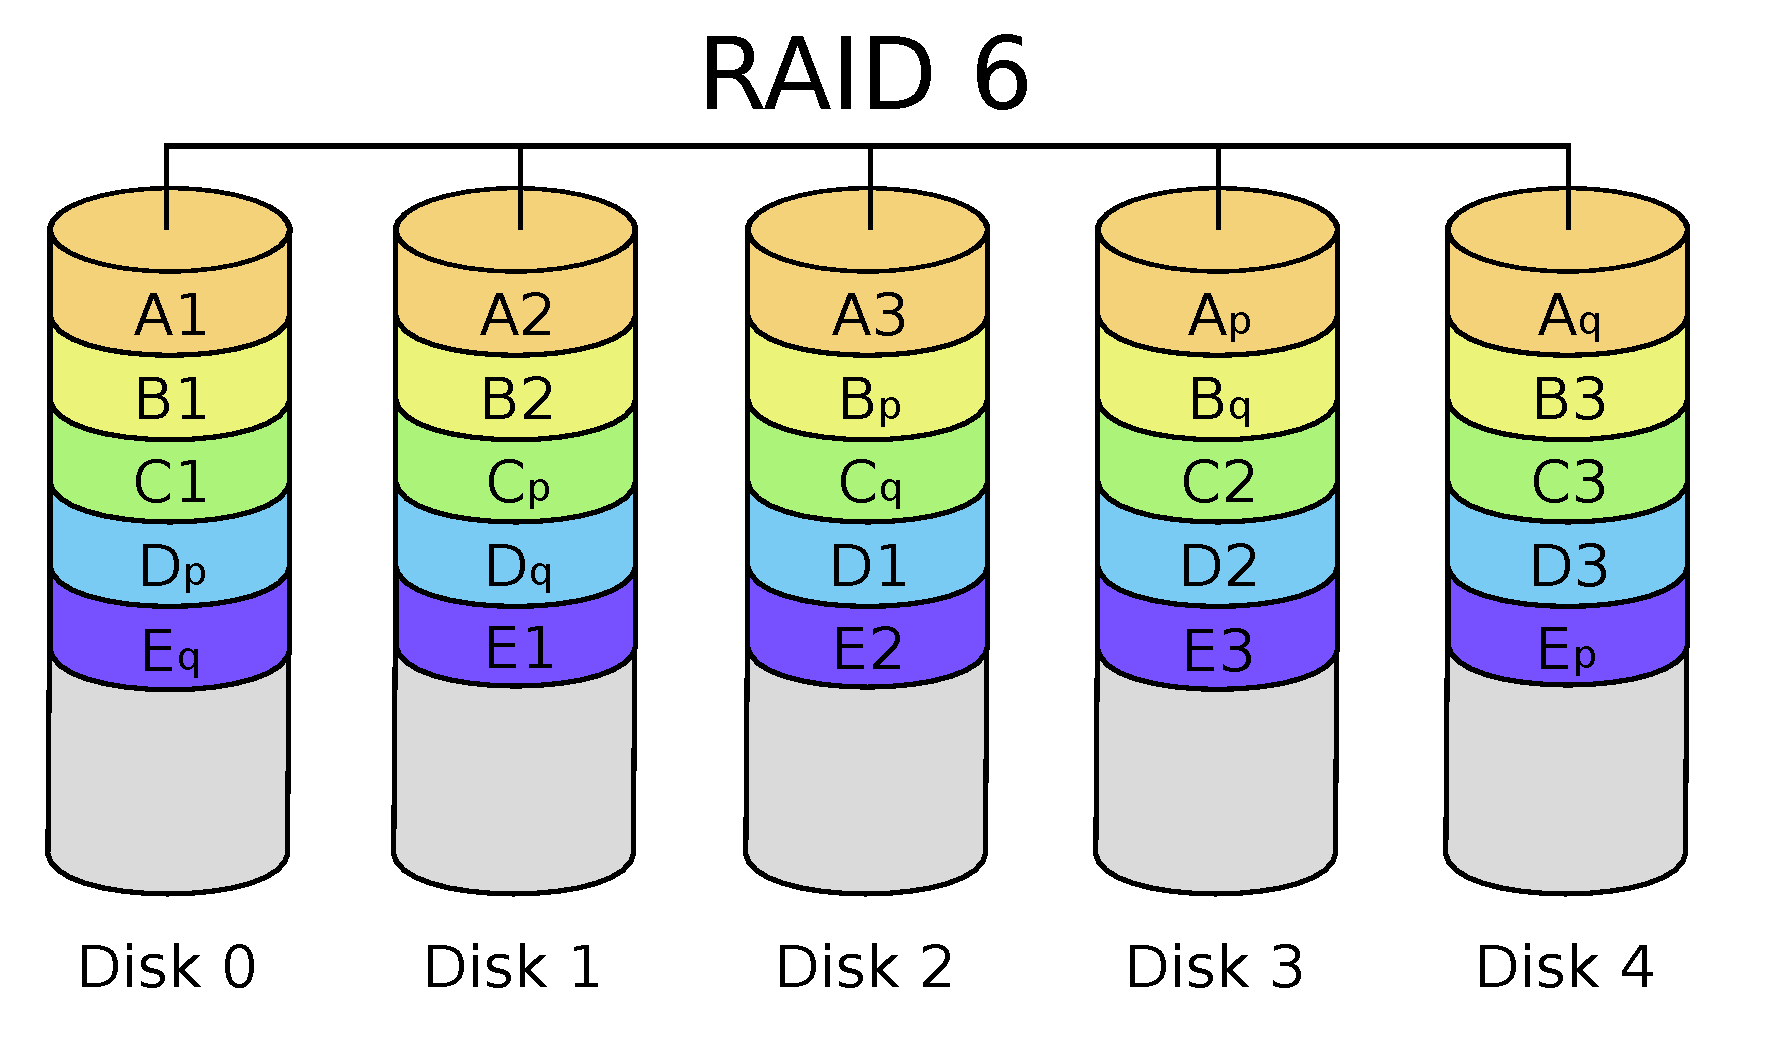
\includegraphics[width=0.9\columnwidth]{/RAID_6}
\end{columns}
\end{frame}

\begin{frame}{RAID}%{Redundant Array of Independent/Inexpensive Disks}

%~ \begin{block}{\small RAID 0+1}
\begin{columns}
\column{.5\textwidth}<1->
\centering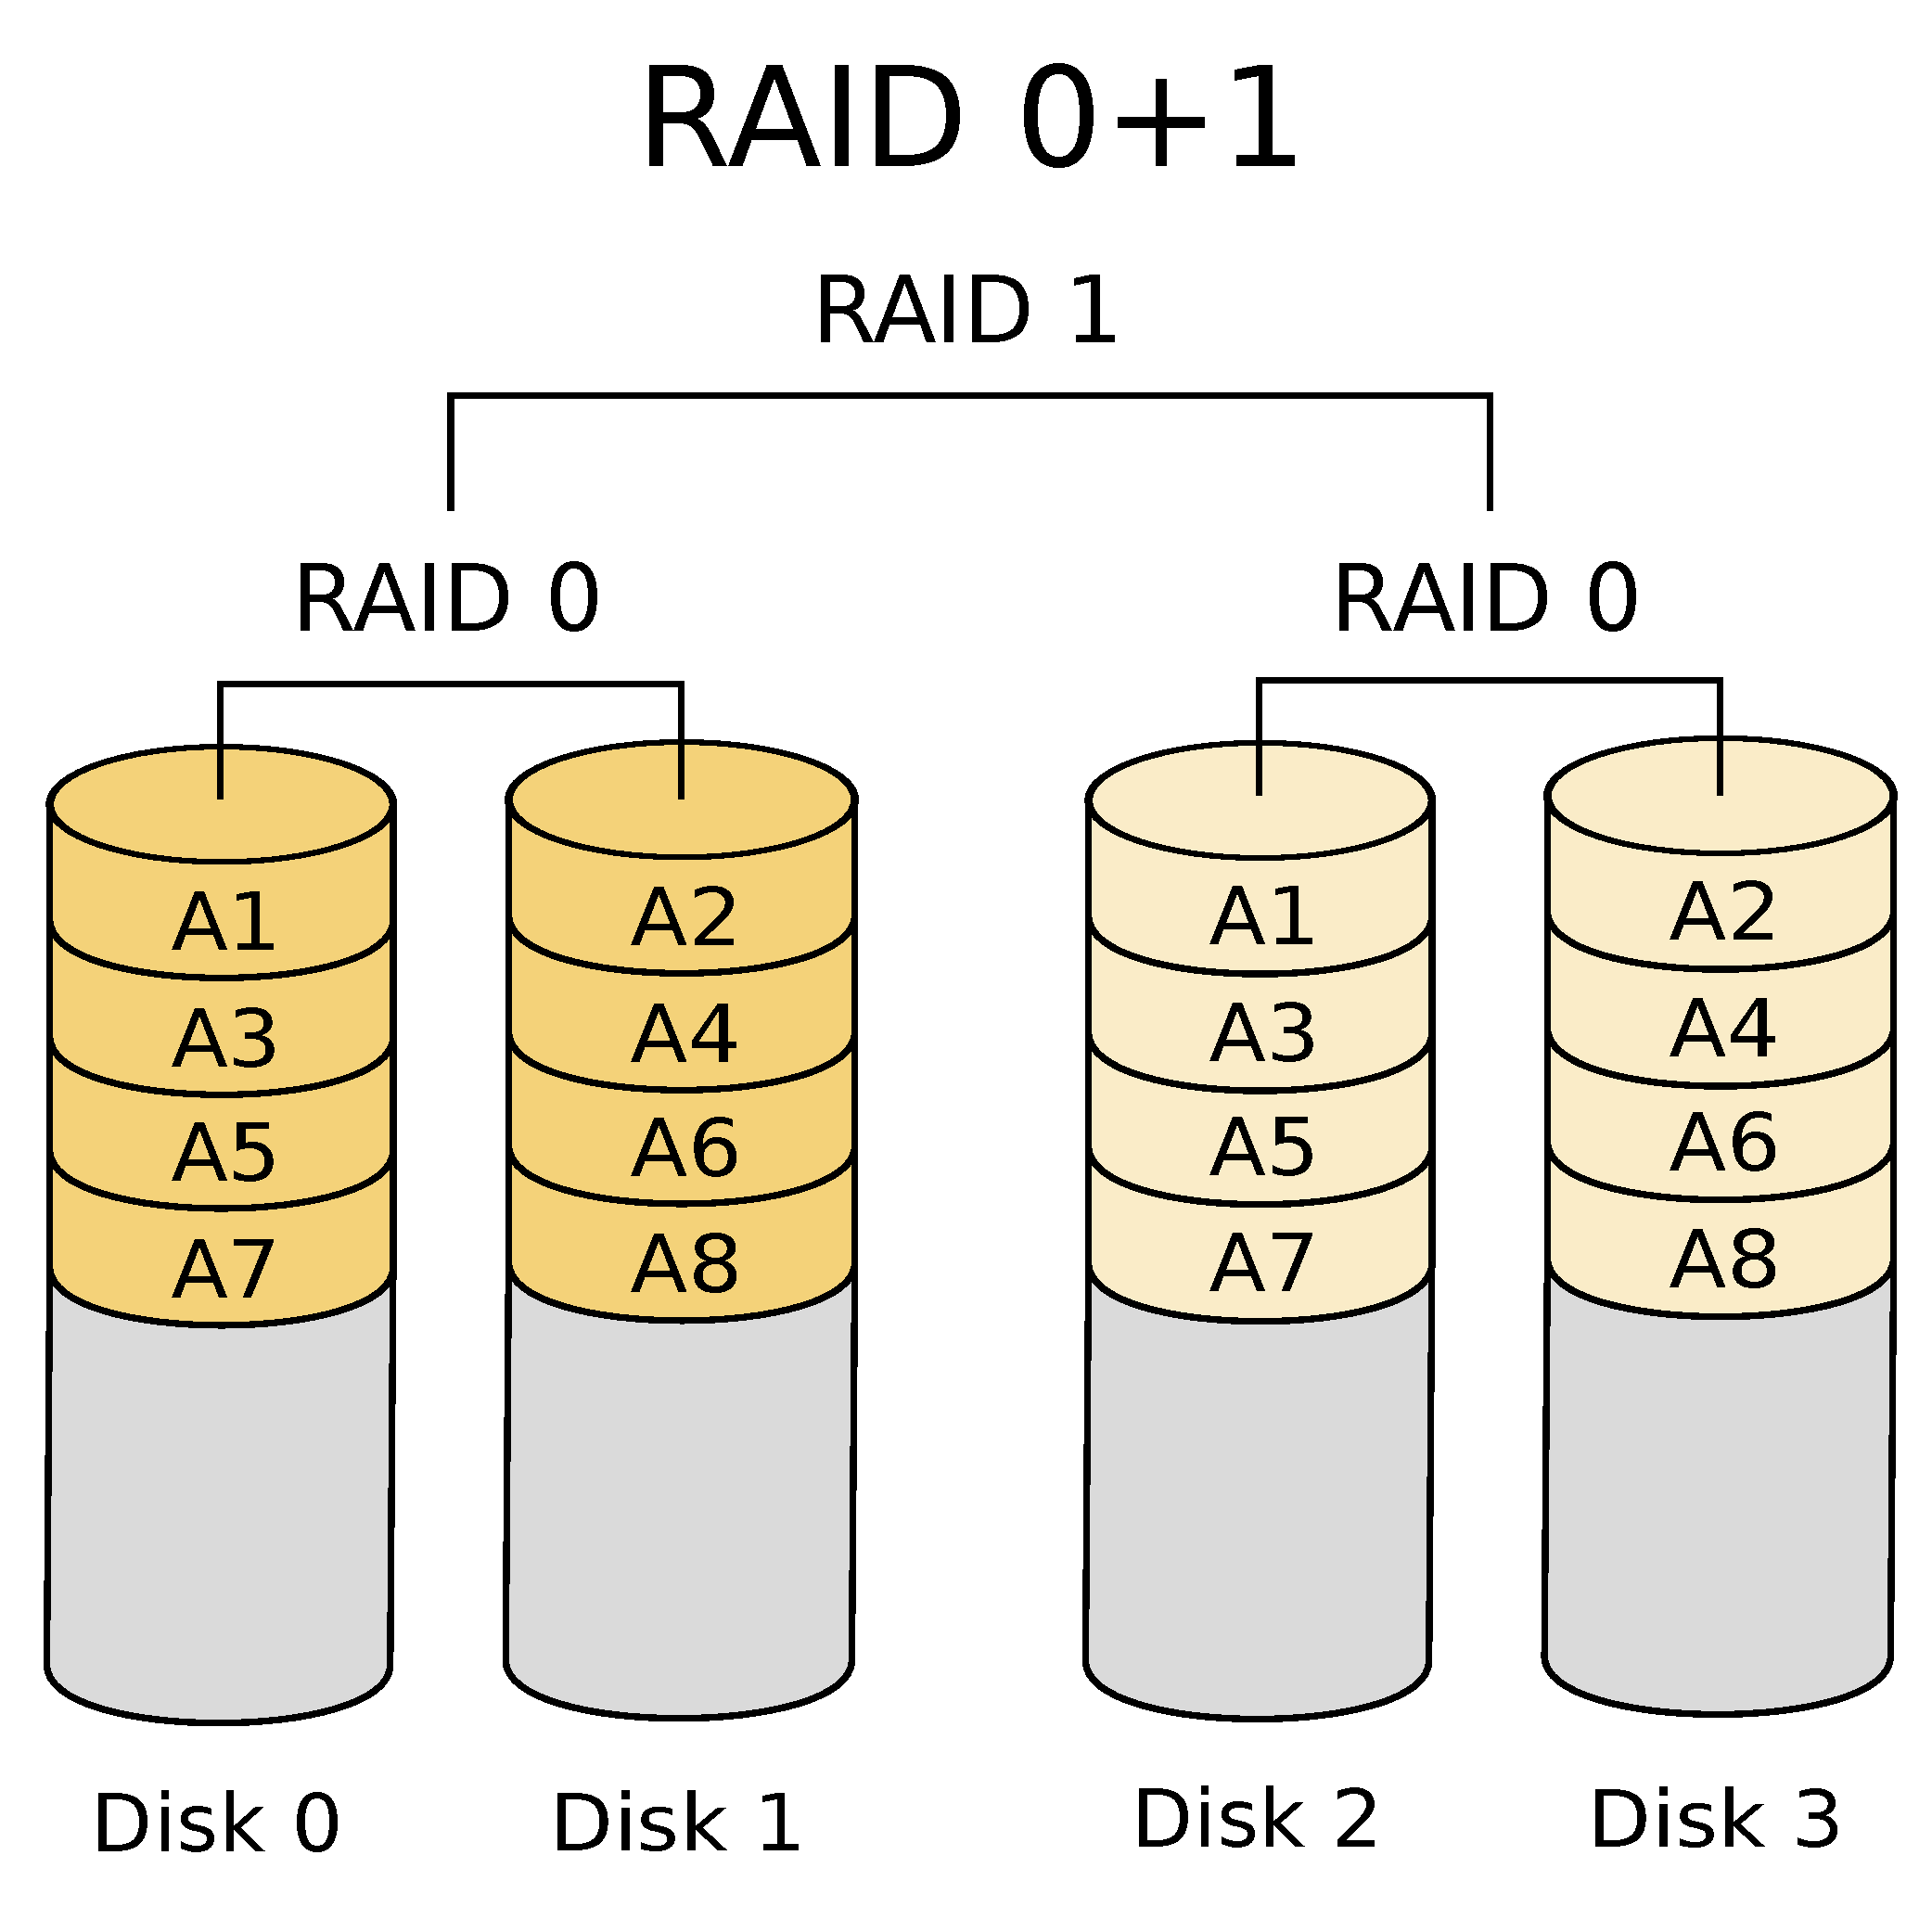
\includegraphics[width=0.9\columnwidth,height=0.44\textheight,keepaspectratio=true]{/RAID_01}
%~ \column{.5\textwidth}
%~ \centering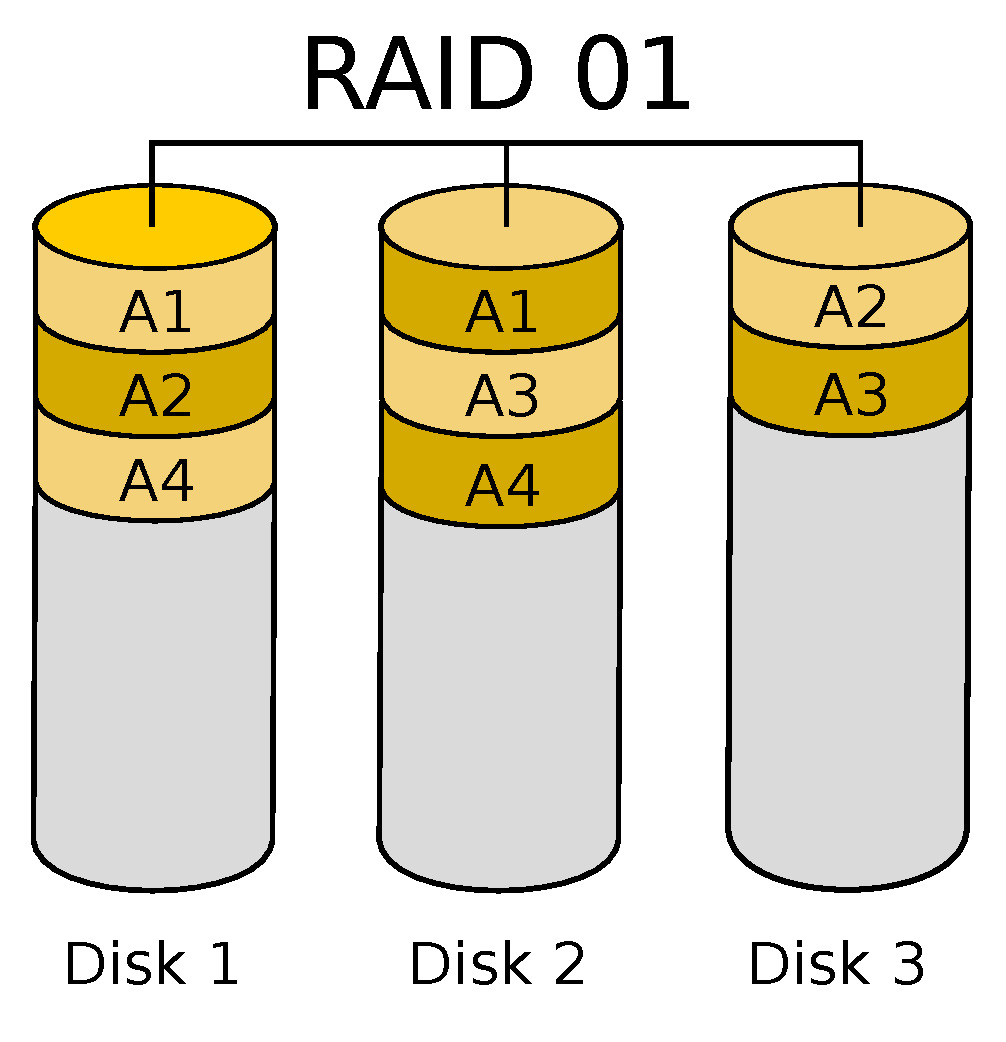
\includegraphics[width=0.9\columnwidth,height=0.33\textheight,keepaspectratio=true]{/RAID_01-3}
\end{columns}
%~ \end{block}
%~ \begin{block}{\small RAID 1+0}
\begin{columns}
\column{.5\textwidth}<2->
\centering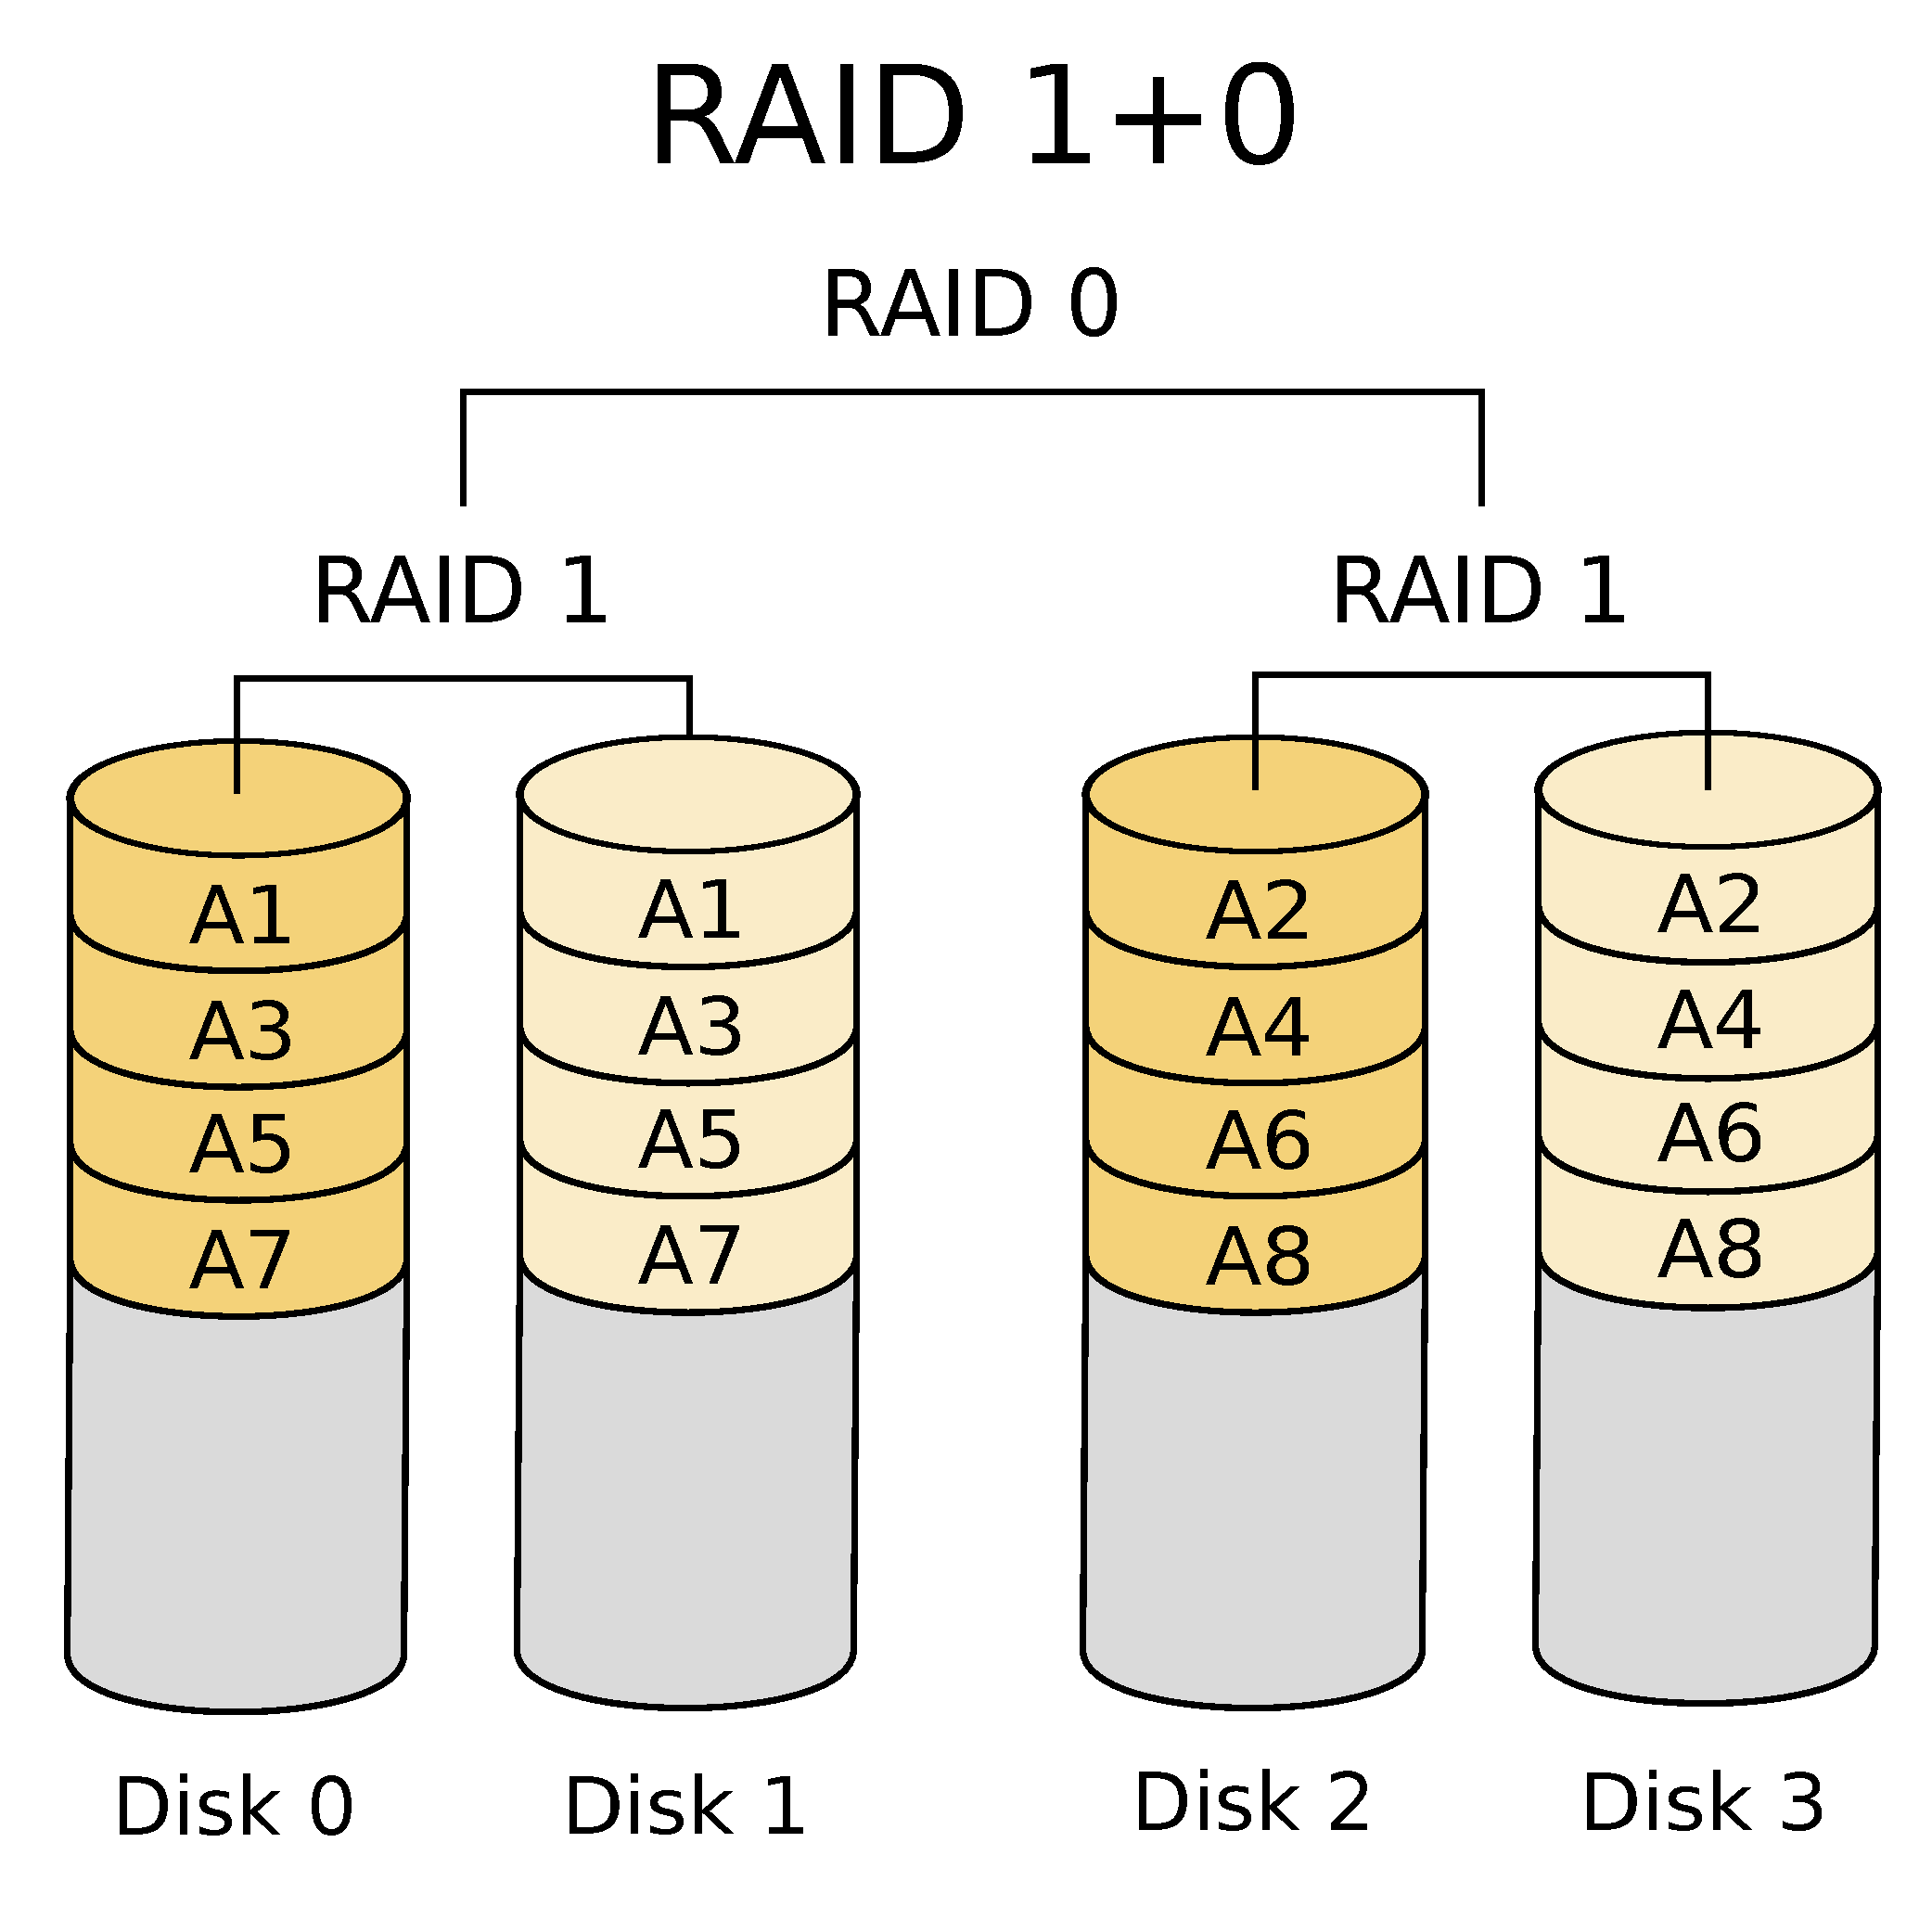
\includegraphics[width=0.9\columnwidth,height=0.44\textheight,keepaspectratio=true]{/RAID_10}
\column{.5\textwidth}<3->
\centering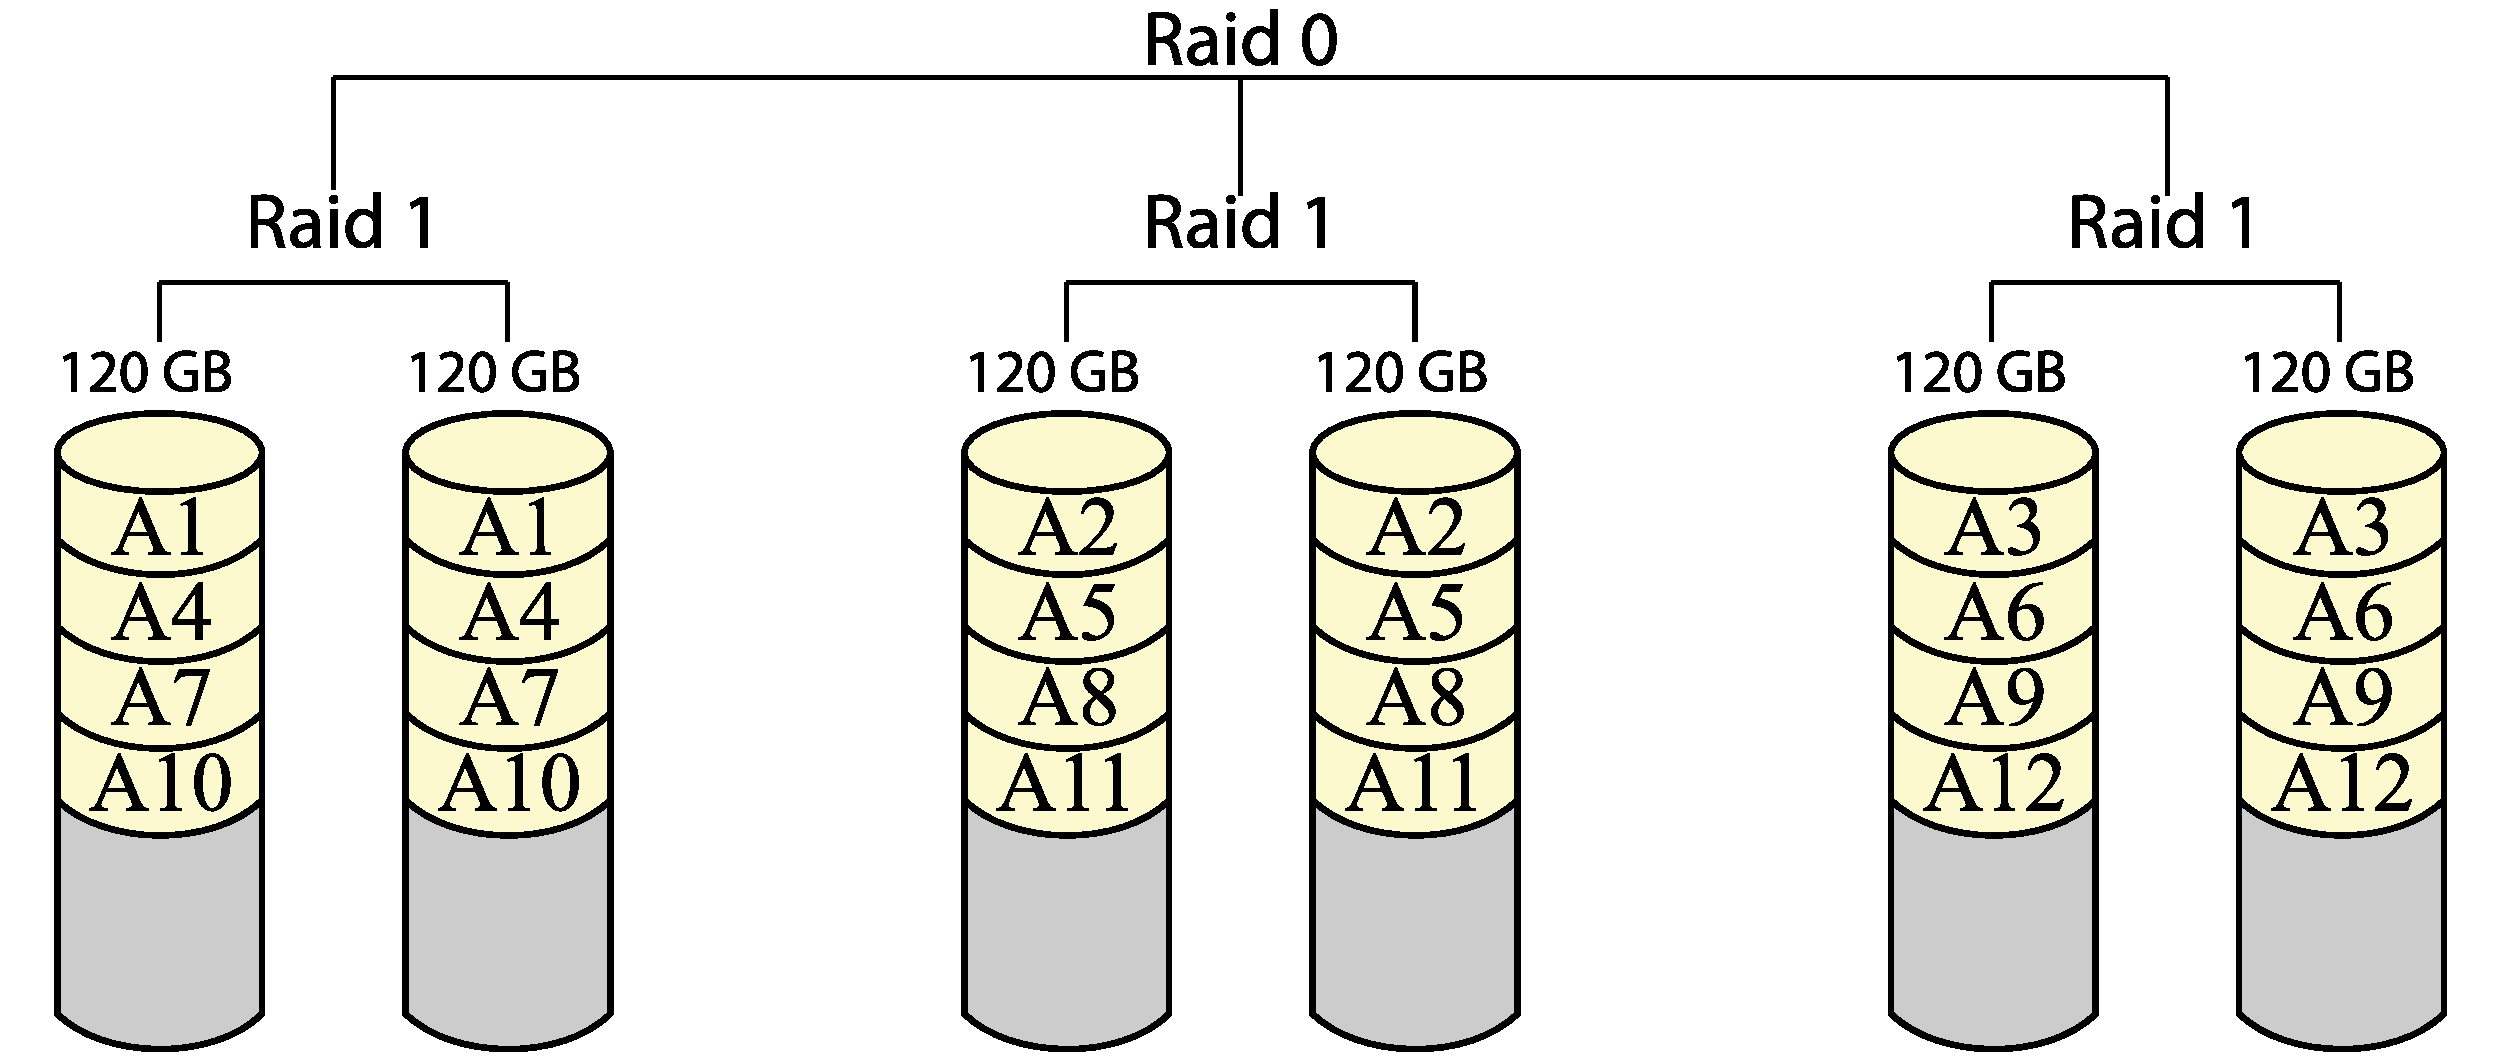
\includegraphics[width=0.9\columnwidth,height=0.44\textheight,keepaspectratio=true]{/RAID_10_6Drives}
\end{columns}
%~ \end{block}
\end{frame}

\begin{frame}{RAID}{Redundant Array of Independent/Inexpensive Disks}
\centering\small
\begin{tabular}{| c || c | c | c |} \hline
RAID-Level & $n$ {\footnotesize(Anzahl Festplatten)} & $k$ {\footnotesize(Nettokapazität)} & $S$ {\footnotesize(Ausfallsicherheit)} \\
\hline
0 & $ \geq 2 $ & $n$ & $0$ \\
1 & $ \geq 2 $ & $1$ & $n \minus 1$ \\
4 & \multirow{2}{*}{$ \geq 3 $} & \multirow{2}{*}{$n \minus 1$} & \multirow{2}{*}{$1$} \\
5 & & & \\
6 & $ \geq 4 $ & $n \minus 2$ & $2$ \\
\hline
\multirow{2}{*}{1+0} & \multirow{2}{*}{$ i \times j $ ($i,j \geq 2 $)} &
\multirow{2}{*}{$\frac{n}{2}$} & $S_{min}=i \minus 1$ \\
& & & $S_{max}=j(i \minus 1)=ji \minus j$ \\
\multirow{2}{*}{0+1} & \multirow{2}{*}{$ i \times j $ ($i,j \geq 2 $)} &
\multirow{2}{*}{$\frac{n}{2}$} & $S_{min}=j \minus 1$ \\
& & & $S_{max}=(j \minus 1)i=ji \minus i$ \\
\hline
\vdots & \vdots & \vdots & \vdots \\
\hline \end{tabular}

\end{frame}

\demo{}
\note{
\texttt{\scriptsize%
\\\$ ls -l /dev/vd*
\\\$ fdisk -l /dev/vdb
\\\$ cat /proc/mdstat
\\\$ mdadm -\--create --help
\\\$ mdadm -\--create /dev/md1 -\--level=6 -\--raid-devices=6 /dev/vd[bcdefg]1
\\\$ cat /proc/mdstat
\\\$ mdadm -\--query /dev/vdb1
\\\$ mdadm -\--query /dev/md1
\\\$ mdadm -\--examine /dev/vdb1
\\\$ mdadm -\--detail /dev/md1
\\\$ mdadm -\--create /dev/md1 -\--level=6 -\--raid-devices=5 -\--spare-devices=1 /dev/vd[bcdefg]1
\\\$ cat /proc/mdstat
\\\$ mdadm -\--detail /dev/md1
}\\ \textbackslash{}o/}

\subsection{LVM}

\begin{frame}{LVM}{Logical Volume Manager}
\begin{block}{LVM}
\begin{itemize}
	\item Physical Volumne
	\item Volume Group
	\item Logical Volume
\end{itemize}
\end{block}
\end{frame}

\begin{frame}[plain]%{LVM}{Logical Volume Manager}
%~ \begin{block}{LVM}
	\centering\colorbox{white}{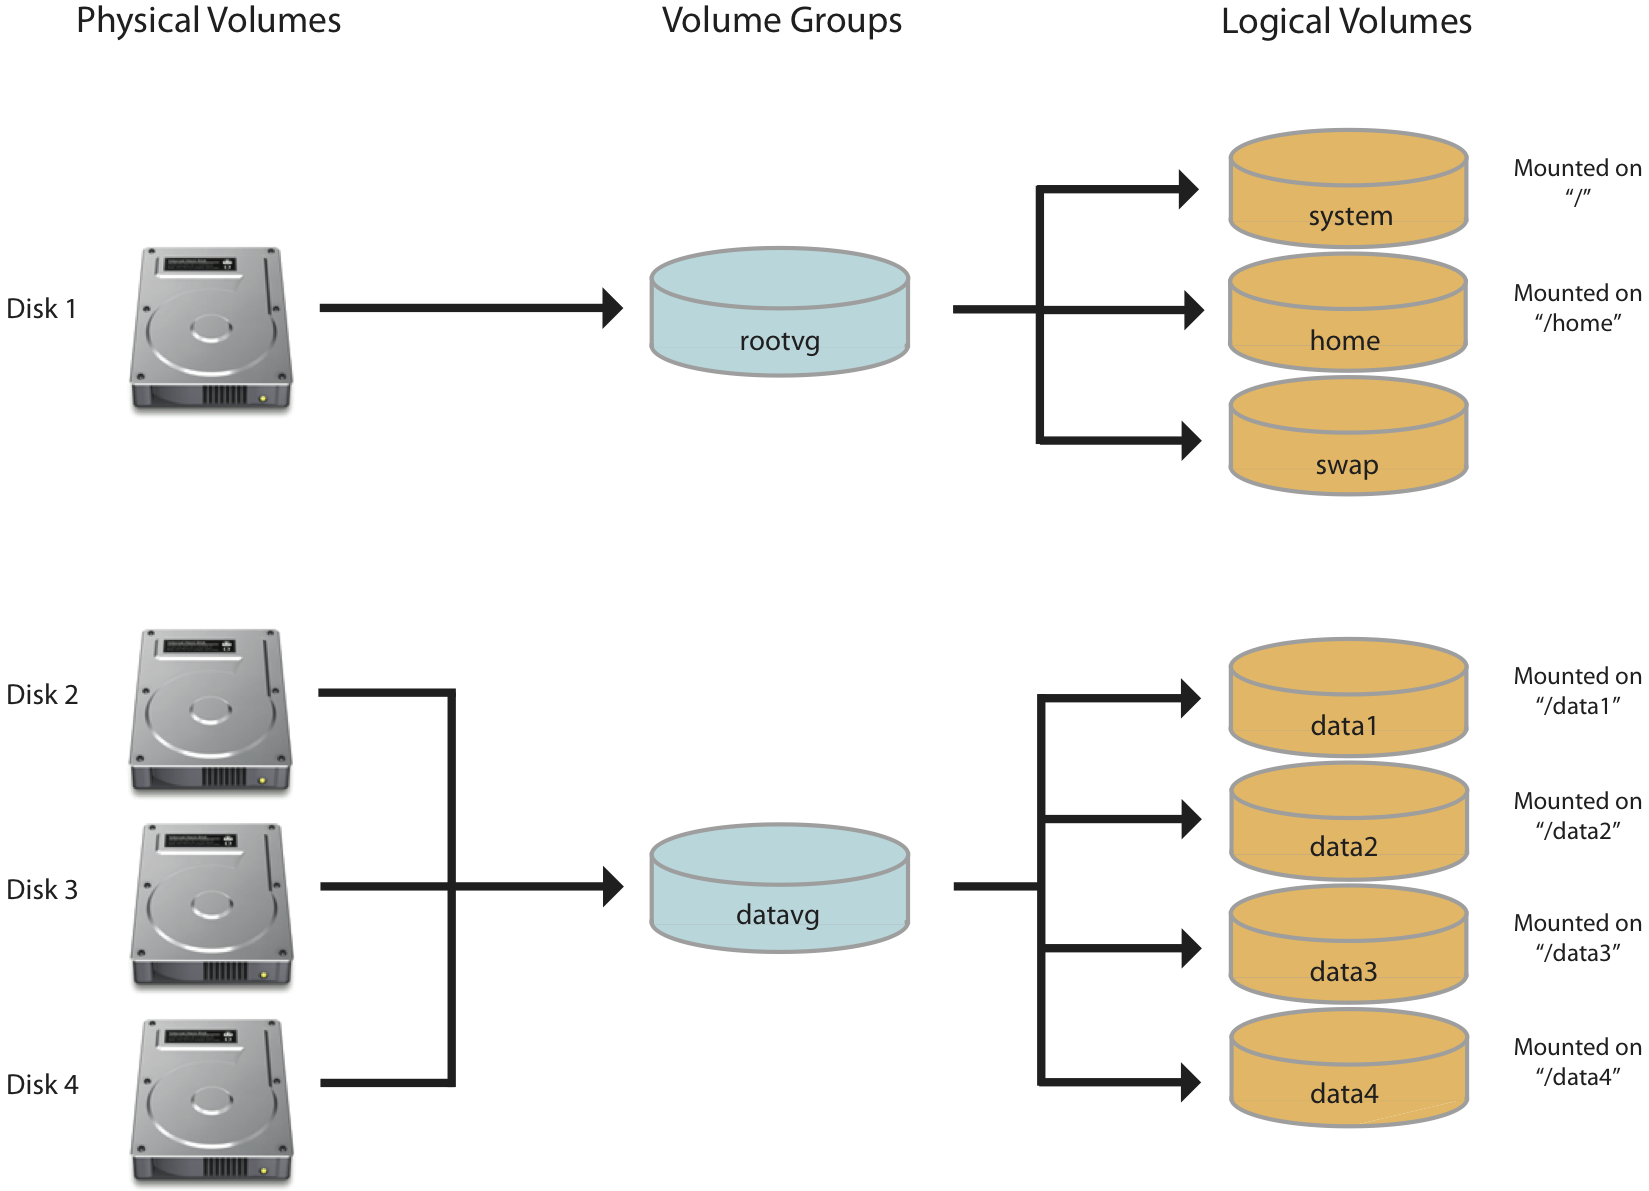
\includegraphics[height=0.9\textheight]{LVM}}

   	\flushleft{\tiny
   	%~ File:Unix history-simple.svg, Revision as of 17:10, 23 June 2012 --
   	%~ Source: Wikimedia Commons, License: CC-BY-SA-3.0\\
   	URL: \url{http://www.helios.de/support/manuals/vsa-e/volume-management.html}
   	}
%~ \end{block}
\end{frame}

\begin{frame}[plain]%{LVM}{Logical Volume Manager}
%~ \begin{block}{LVM on RAID}
	\centering\colorbox{white}{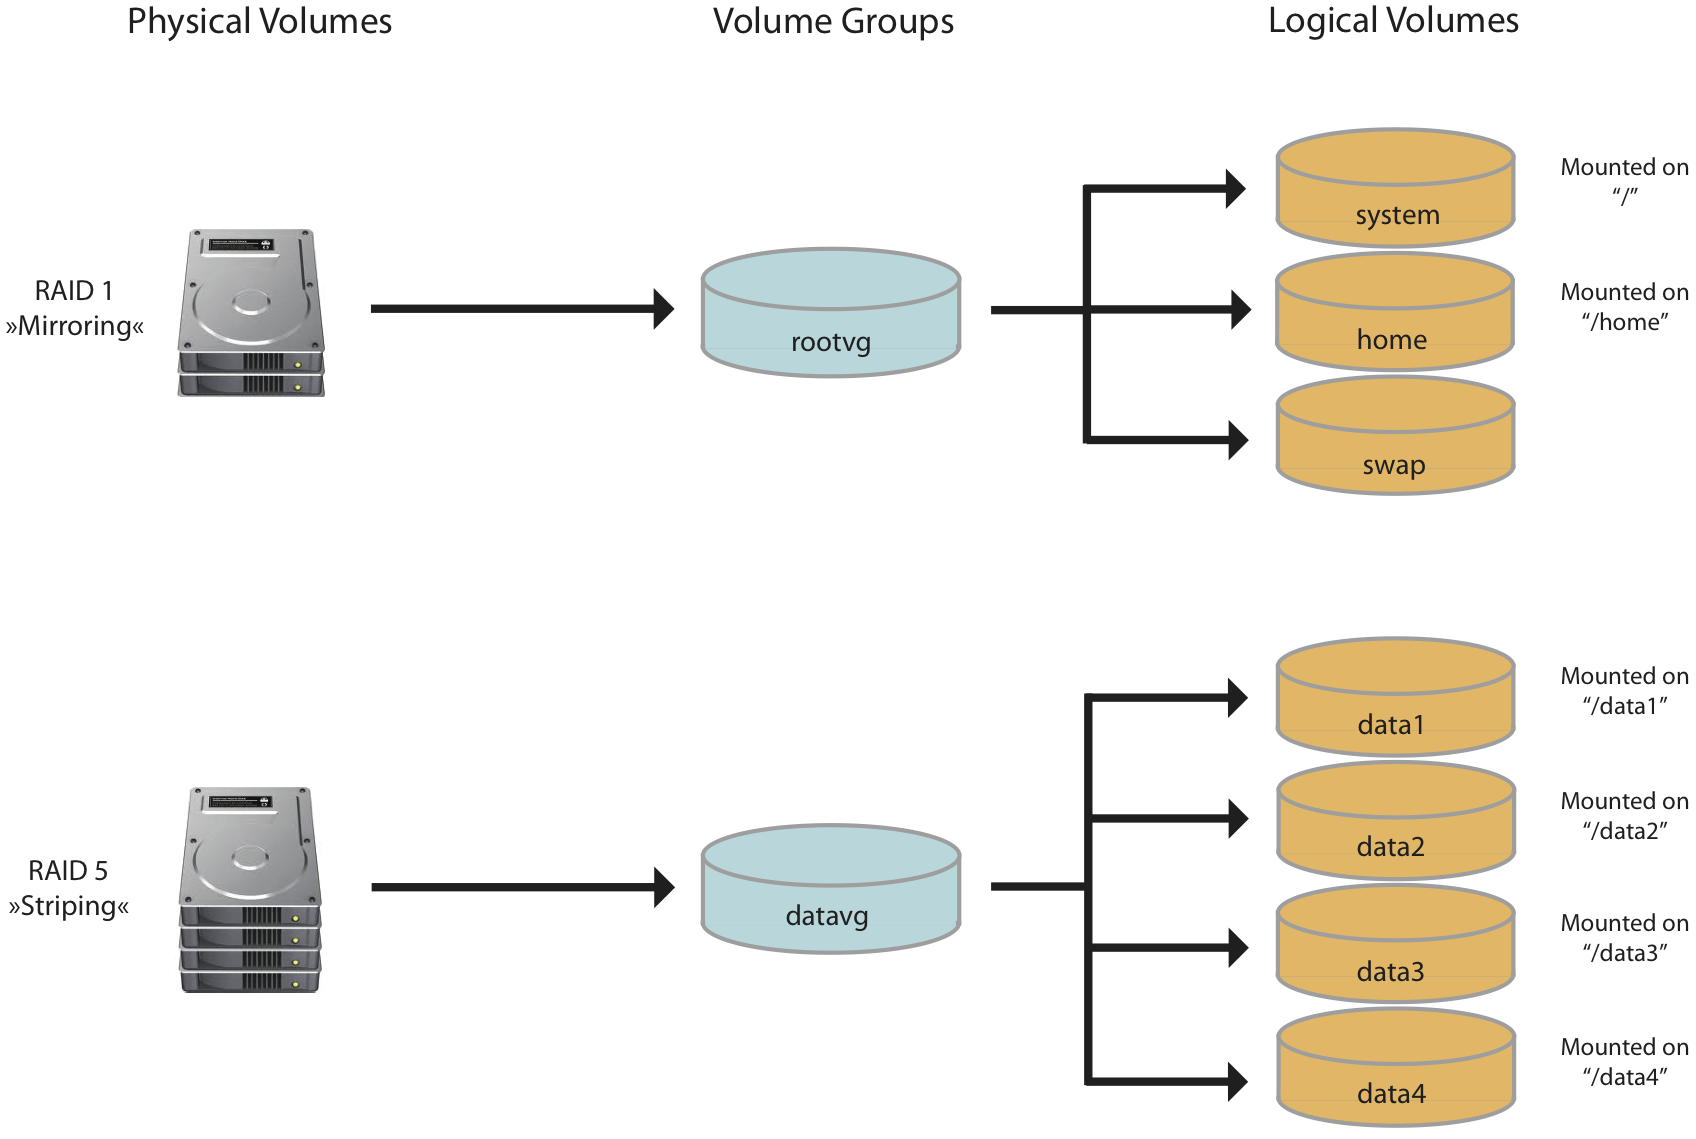
\includegraphics[height=0.9\textheight]{LVM-RAID}}

   	\flushleft{\tiny
   	%~ File:Unix history-simple.svg, Revision as of 17:10, 23 June 2012 --
   	%~ Source: Wikimedia Commons, License: CC-BY-SA-3.0\\
   	URL: \url{http://www.helios.de/support/manuals/vsa-e/volume-management.html}
   	}
%~ \end{block}
\end{frame}

\demo{}
\note{
\texttt{\scriptsize%
\\\$ mdadm -\--create /dev/md1 -\--level=1 -\--raid-devices=2 /dev/vd[bc]1
\\\$ mdadm -\--create /dev/md2 -\--level=1 -\--raid-devices=2 /dev/vd[de]1
\\\$ mdadm -\--create /dev/md3 -\--level=1 -\--raid-devices=2 /dev/vd[fg]1
\\\$ cat /proc/mdstat
\\\$ pvcreate -h
\\\$ pvcreate /dev/md1 /dev/md2 /dev/md3
\\\$ pvs
%~ \\\$ pvscan
\\\$ pvdisplay
\\\$ vgcreate -h
\\\$ vgcreate data /dev/md\{1..3\}
\\\$ vgs
\\\$ vgdisplay
\\\$ lvcreate -h
\\\$ lvcreate -l 100\%FREE -n storage data
\\\$ lvs
\\\$ lvdisplay
}\\ \textbackslash{}o/}

\note{
\texttt{\scriptsize%
\\\$ mkfs.ext4 -L storage /dev/data/storage
\\\$ mount /dev/data/storage /mnt/storage
%~ \\\$ vim /etc/conf.d/mdraid
\\\$ vim /etc/conf.d/lvm
%~ \\\$ rc-update add mdraid boot
\\\$ rc-update add lvm boot
\\\$ reboot
}\\ \textbackslash{}o/}

\subsection{LUKS}

\begin{frame}{LUKS}{Linux Unified Key Setup}
\centering
\includegraphics[width=0.33\columnwidth]{luks-logo}
\begin{block}{LUKS}
\begin{itemize}
	\item dm-crypt
	\item cryptsetup
\end{itemize}
\end{block}
\end{frame}

\begin{frame}[plain]%{LUKS}
%~ \begin{block}{LUKS}
	%~ \centering\colorbox{white}{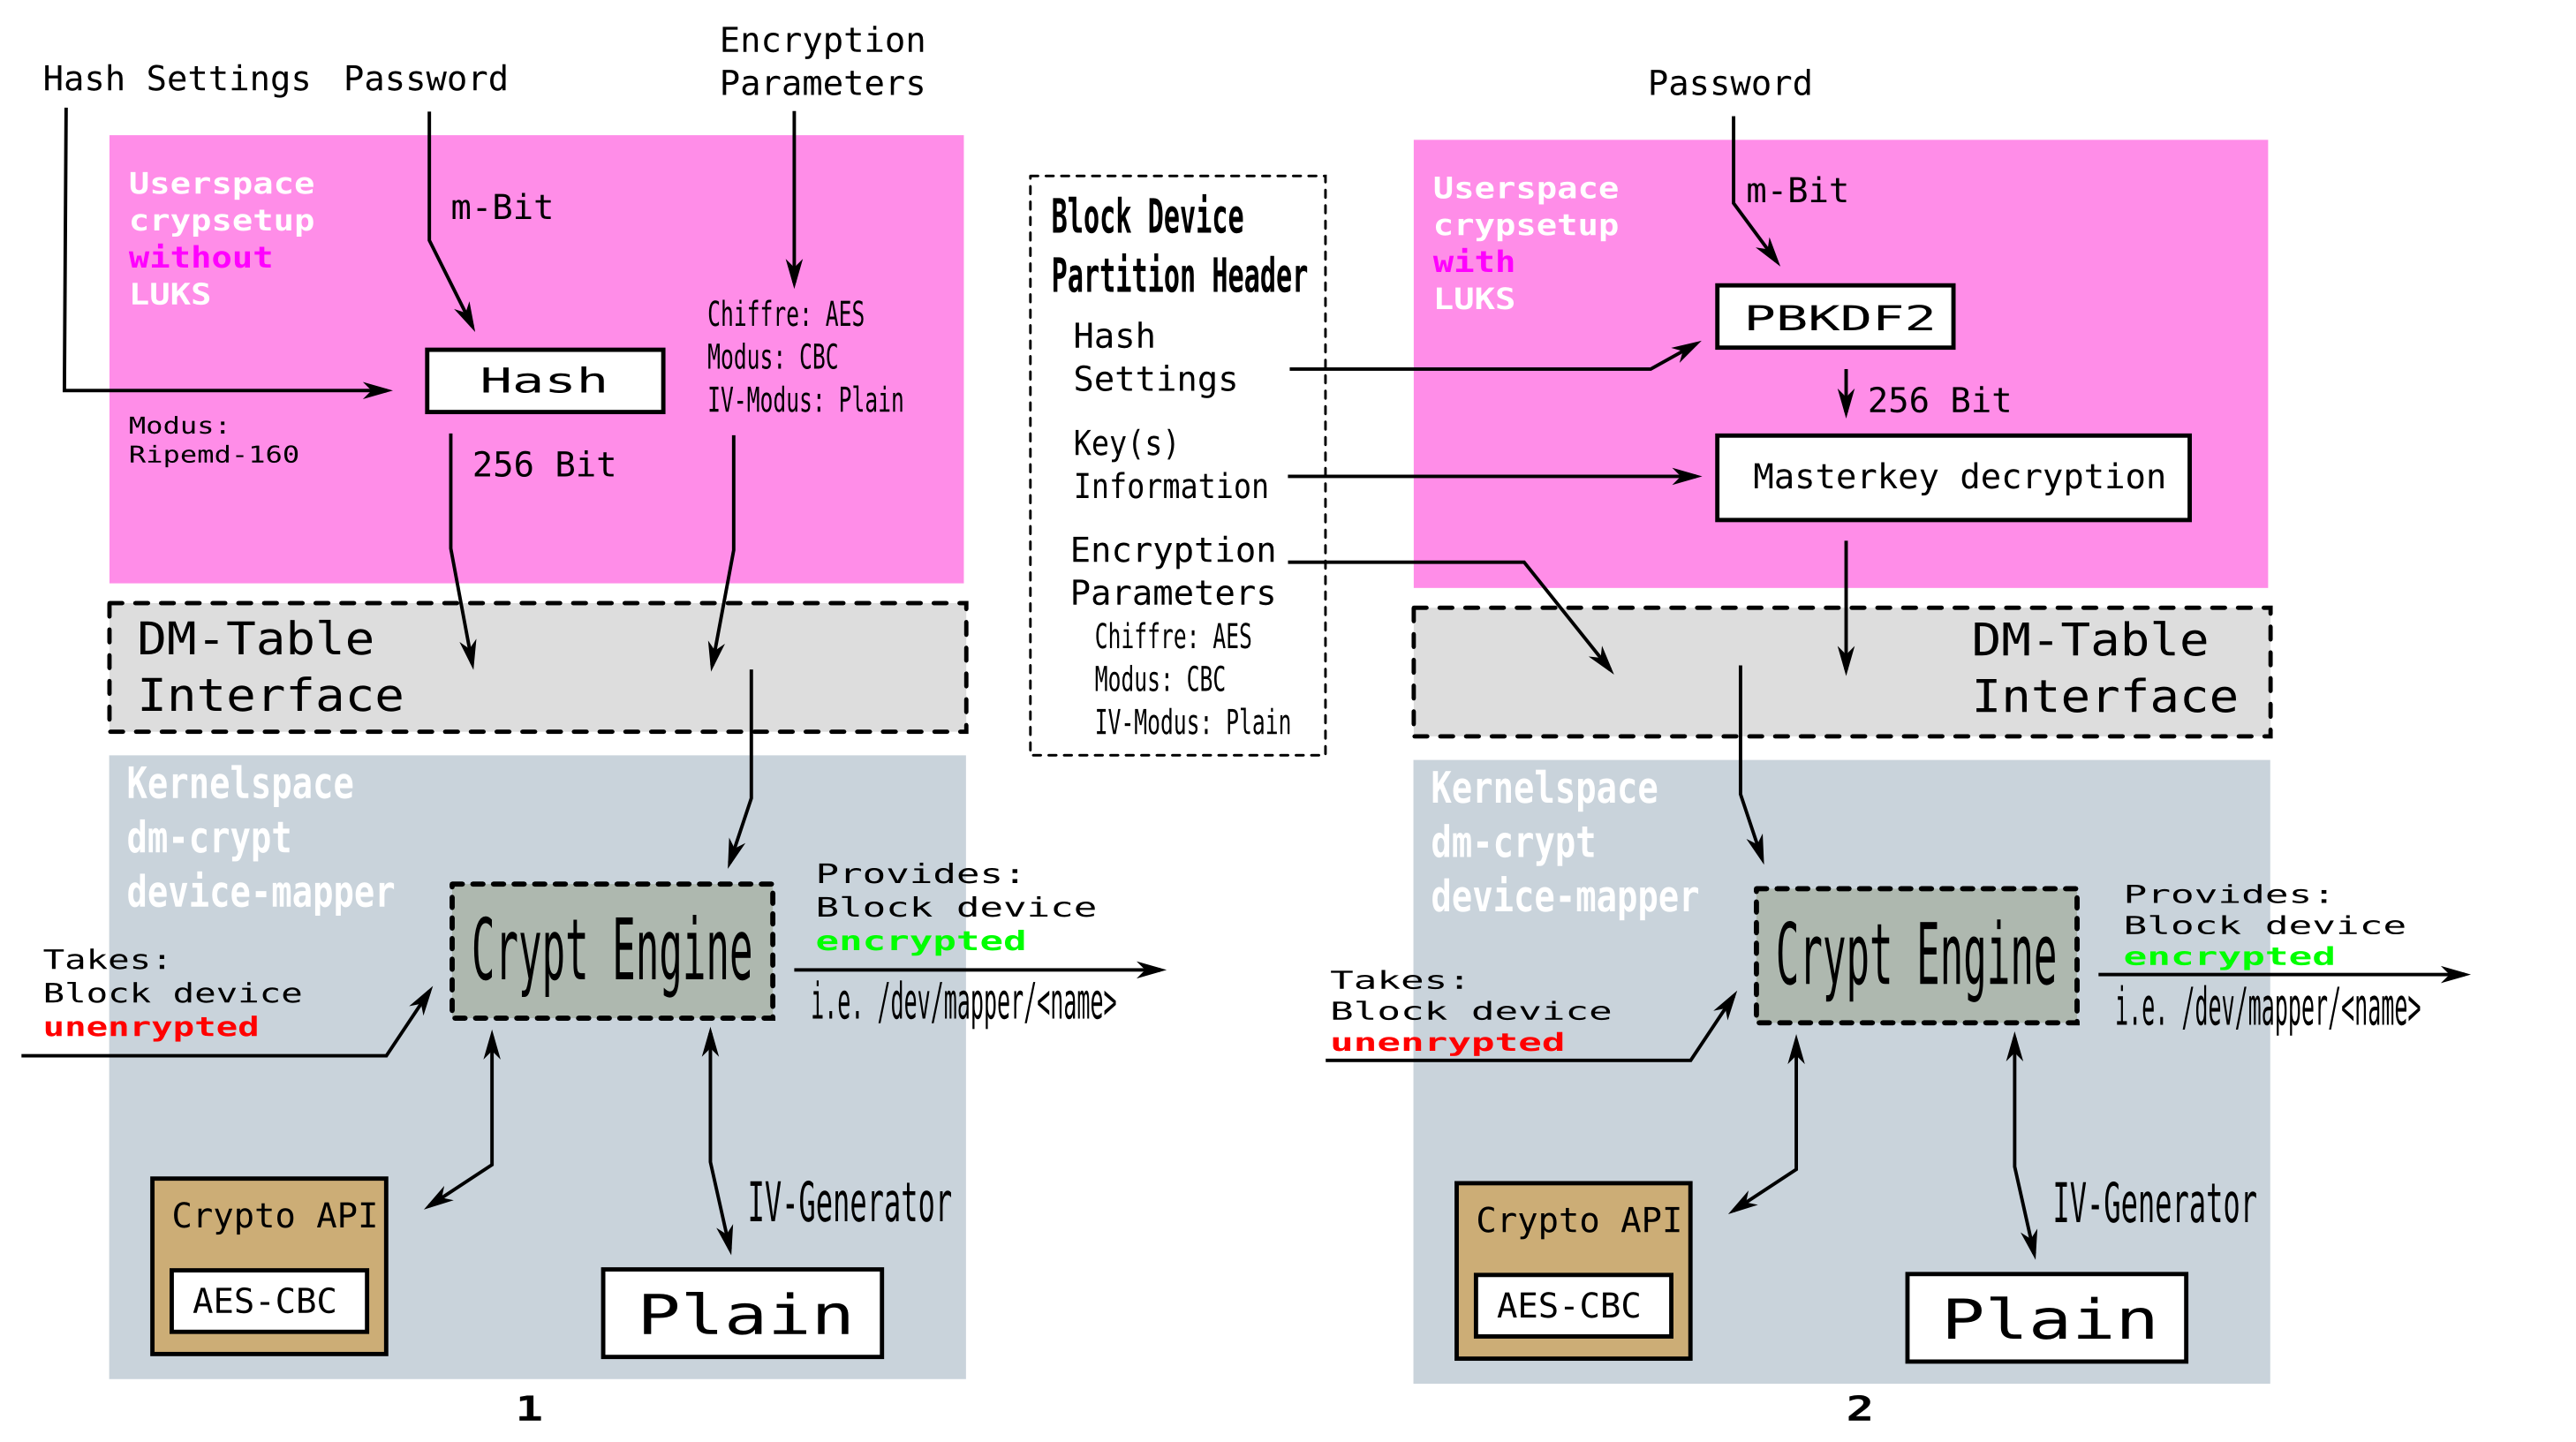
\includegraphics[width=\textwidth]{keys_and_pw_with_luks}}

\mynote{PBKDF2:}{Password-Based Key Derivation Function}

\begin{columns}
\column{.5\textwidth}<1->
\centering\colorbox{white}{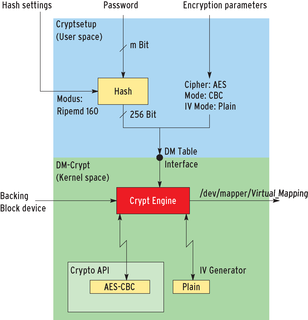
\includegraphics[width=\textwidth]{fig1-regular-cryptsetup_s}}
\flushleft{\tiny Plain cryptsetup}
\column{.5\textwidth}<2->
\centering\colorbox{white}{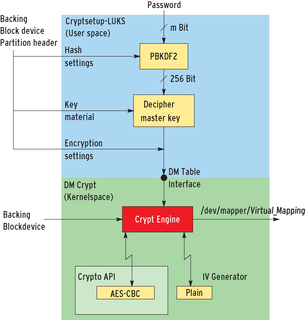
\includegraphics[width=\textwidth]{fig2-luks_s}}
\flushleft{\tiny cryptsetup with LUKS}
\end{columns}

\note{Ohne LUKS keine plausible deniability}

   	\flushleft{\tiny
   	%~ File:Unix history-simple.svg, Revision as of 17:10, 23 June 2012 --
   	%~ Source: Wikimedia Commons, License: CC-BY-SA-3.0\\
   	URL: \url{http://www.markus-gattol.name/ws/dm-crypt_luks.html}
   	}
%~ \end{block}
\end{frame}

\demo{}
\note{
\texttt{\scriptsize%
\\\$ mdadm -\--create /dev/md127 -\--level=6 -\--raid-devices=6 /dev/vd[bcdefg]1
\\\$ cryptsetup luksFormat -q -c aes-xts-plain -s 256 /dev/md127 \~/keyfile
\\\$ cryptsetup luksOpen -d \~/keyfile /dev/md127 enc
\\\$ cat /etc/conf.d/dmcrypt
\\rc\_before="lvm"
\\target=enc
\\source=/dev/md127
\\key=/root/keyfile
\\\$ rc-update add dmcrypt boot
\\\$ pvcreate /dev/mapper/enc
\\\$ vgcreate data /dev/mapper/enc
\\\$ lvcreate -l 100\%FREE -n storage data
}\\ \textbackslash{}o/}

\subsection{ZFS}

\begin{frame}{ZFS}

\begin{block}{Features}
\begin{itemize}
	\item Integrierte RAID- und LVM-Funktionen
	\item Sicherstellung von (Nutz-)Datenintegrität\mynote{avoid data corruption:}{self-healing}
	\item Scrubbing
	\item Copy-on-write
	\begin{itemize}
		\item Transaktionen\mynote{transactional:}{either a write is completely done, or not at all}
		\item Snapshots
	\end{itemize}
	\item Verschlüsselung, Komprimierung
	\mynote{Capacity:}{256 quadrillion zettabytes}
\end{itemize}
\mynote{write hole:}{Zuerst werden Daten geschrieben, dann Paritätsbit}
\end{block}

\end{frame}

\begin{frame}{ZFS}{ZFS on Linux}


\begin{alertblock}{Don't try this at home!}
	ZFS on Linux is experimental software!
\end{alertblock}

\begin{block}{}
	\url{http://zfsonlinux.org/}

	%~ \url{https://mthode.org/posts/2012/Dec/gentoo-hardened-zfs-rootfs-with-dm-cryptluks-updated-2012-12-12/}
\end{block}

\end{frame}

\demo{}
\note{
\texttt{\scriptsize%{}
\\\$ for i in b c d e f g; do
\\\$ cryptsetup luksFormat -q -c aes-xts-plain -s 256 /dev/vd\$\{i\}1 \~/keyfile
\\\$ cryptsetup luksOpen -d \~/keyfile /dev/vd\$\{i\}1 \$\{i\}
\\\$ done
\\\$ zpool create tank raidz2 /dev/mapper/[bcdefg]
\\\$ zfs create -o mountpoint=/mnt/storage/public tank/public
\\\$ zfs create -o mountpoint=/mnt/storage/private tank/private
\\\$ cat /etc/conf.d/zfs
\\rc\_after="dmcrypt"
\\\$ rc-update add zfs boot
}\\ \textbackslash{}o/}

\section{Verteilte Dateisysteme}

\subsection{CIFS (Samba)}

\begin{frame}{CIFS}{Common Internet File System}

%~ \begin{columns}
%~ \column{.45\textwidth}
\begin{block}{}
  \begin{itemize}
    \item Erweiterung von SMB (Server Message Block) -- Namensgeber für Samba
  \end{itemize}
\end{block}
%~ \end{columns}

\end{frame}

\subsection{NFS}

\begin{frame}{NFS}{Network File System}
\begin{block}{}
  \begin{itemize}
    \item NFSv3
    \item NFSv4
  \end{itemize}
\end{block}
\end{frame}

%~ \section{Blick über den Tellerrand}
%~
%~ \subsection{UNIX}
%~
%~ \begin{frame}[plain]%{UNIX}
%~ \begin{block}{UNIX Family Tree}
	%~ \centering\colorbox{white}{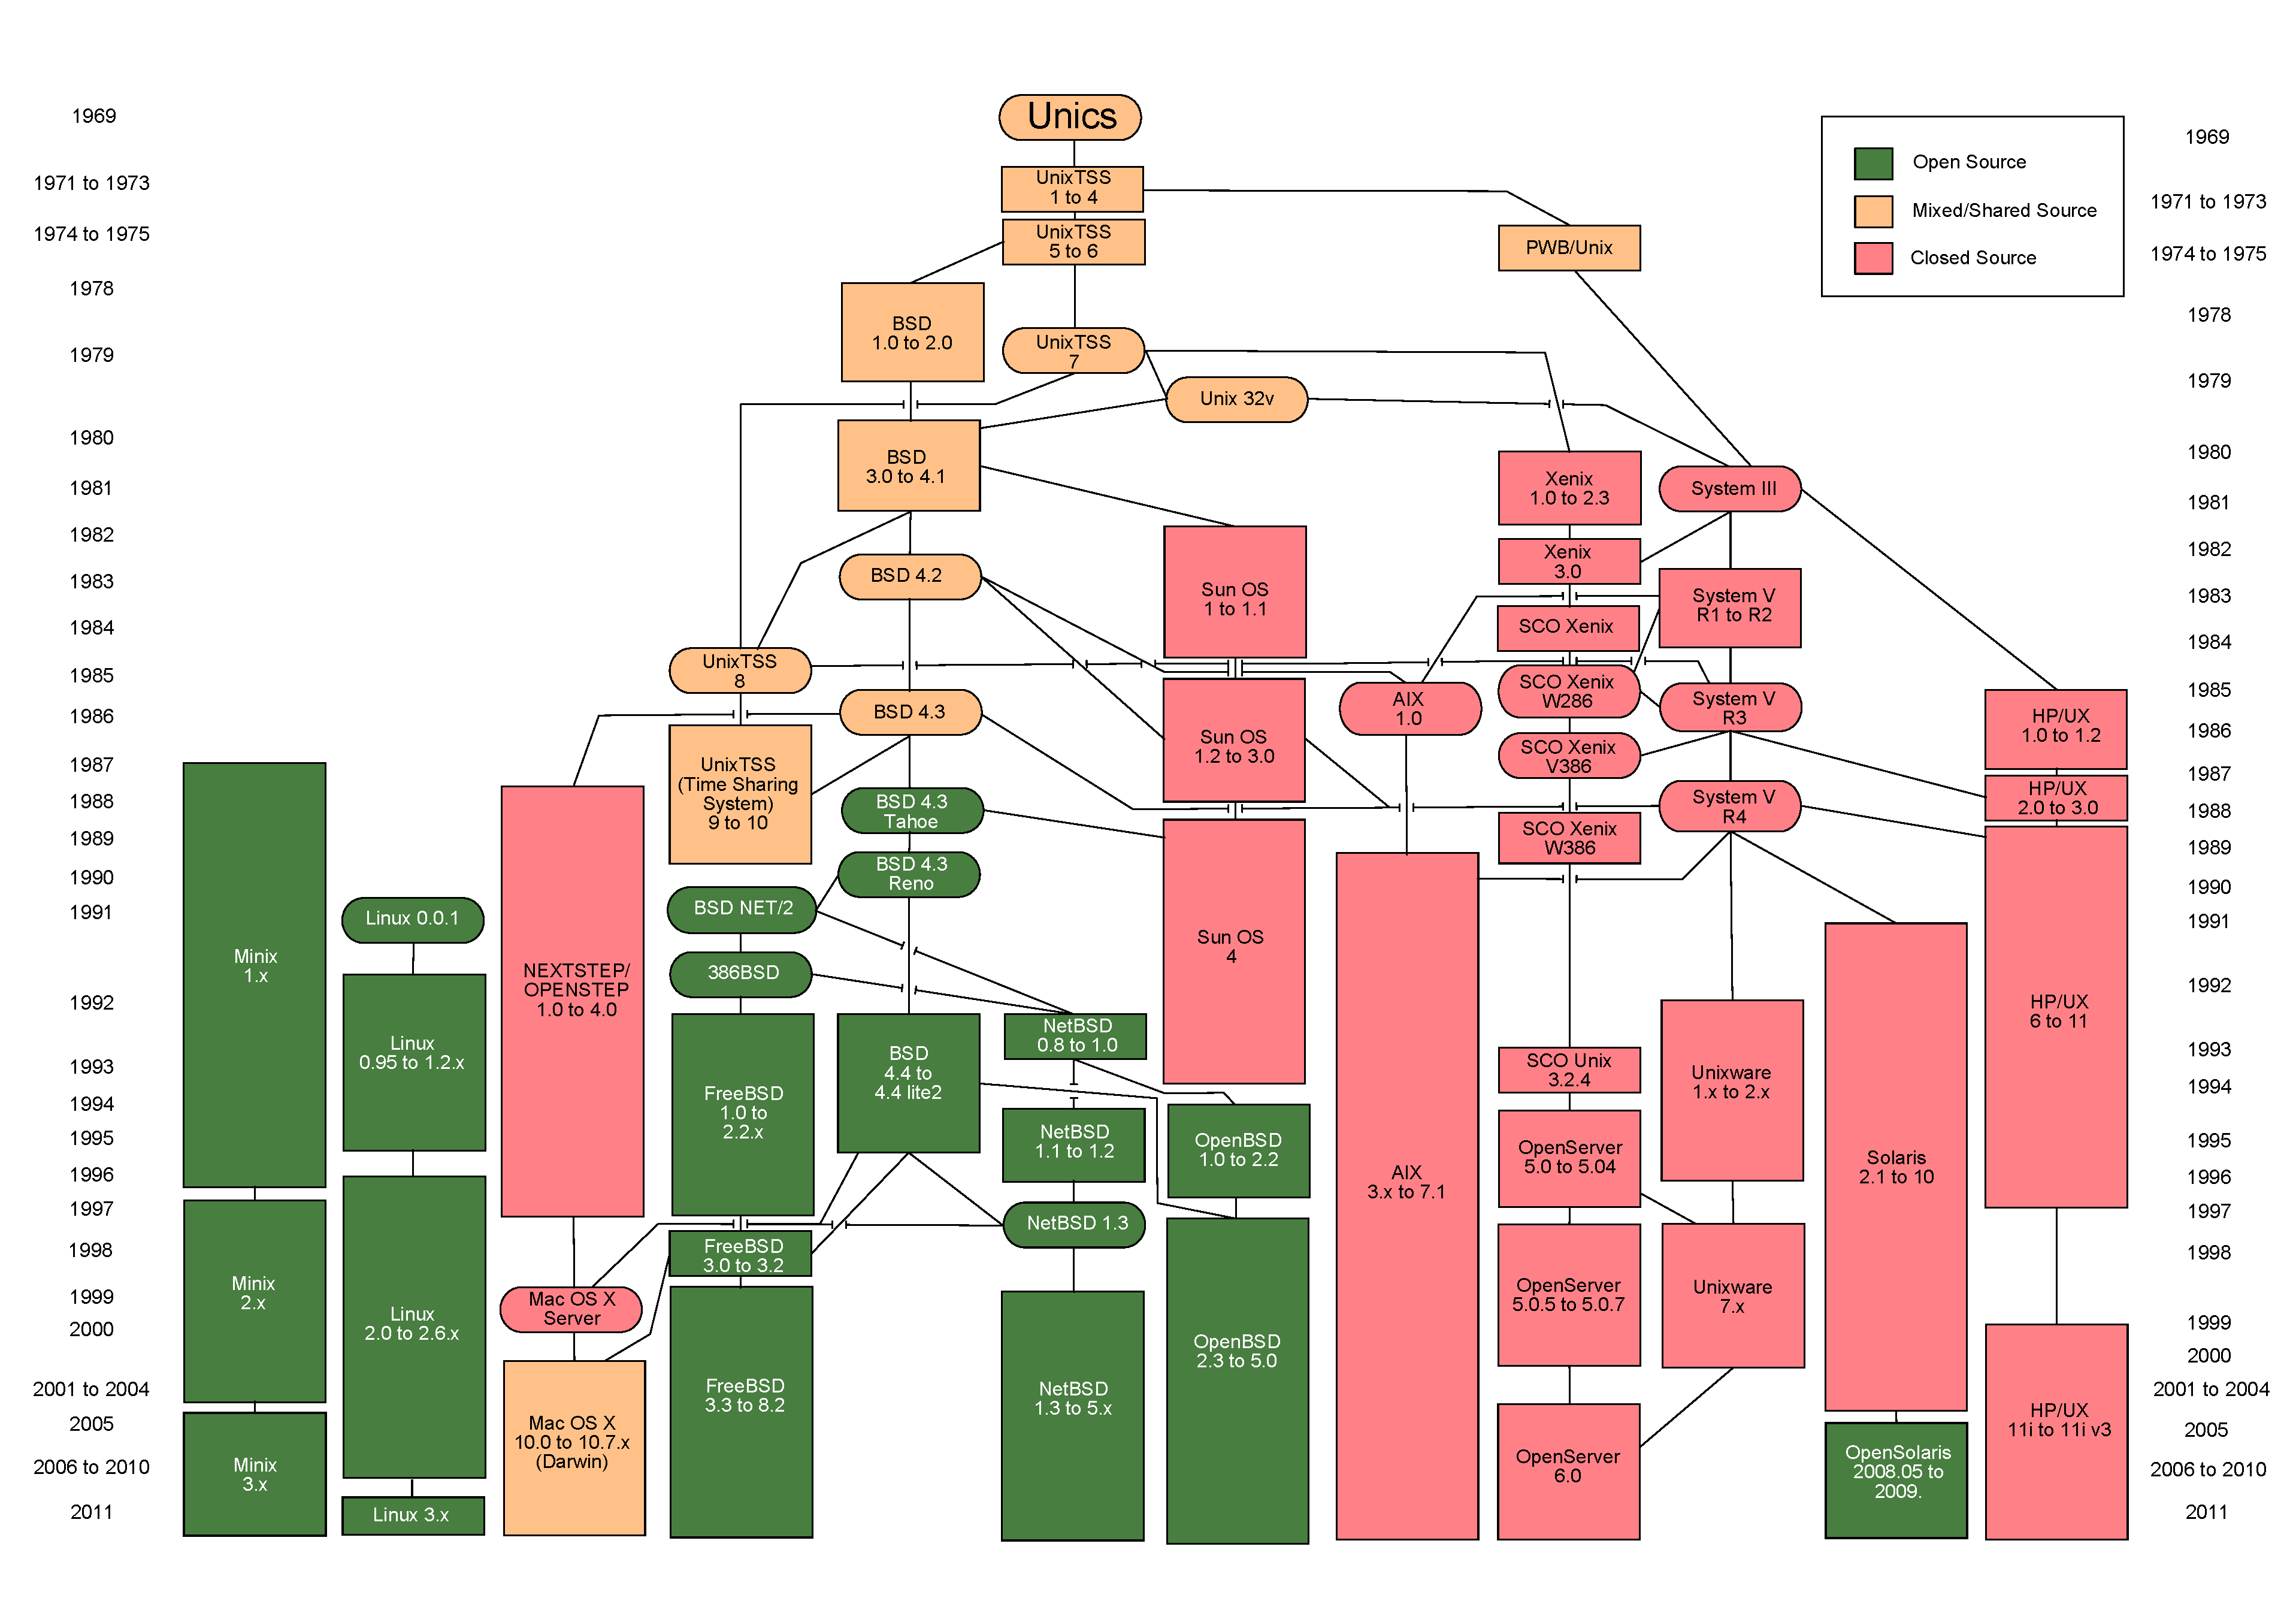
\includegraphics[height=0.9\textheight]{Unix_history-simple}}
%~
   	%~ \flushleft{\tiny File:Unix history-simple.svg, Revision as of 17:10, 23 June 2012 --
   	%~ Source: Wikimedia Commons, License: CC-BY-SA-3.0 \\
   	%~ URL: \url{http://commons.wikimedia.org/w/index.php?title=File:Unix_history-simple.svg&oldid=73135501}
   	%~ }
%~ \end{block}
%~ \end{frame}
%~
%~ \subsection{Lizenzen}
%~
%~ \begin{frame}{GPL vs. the Rest}
%~ \begin{columns}
%~ \column{.45\textwidth}
%~ \centering
\includegraphics[width=0.5\columnwidth]{Official_gnu}
%~ \column{.45\textwidth}
%~ \centering
\includegraphics[width=0.5\columnwidth]{GPLv3_Logo}
%~ \end{columns}
%~ \begin{columns}
%~ \column{.45\textwidth}
%~ \begin{block}{GPL-kompatibel}
  %~ \begin{itemize}
    %~ \item LGPL
    %~ \item BSD-2, BSD-3
    %~ \item MIT
  %~ \end{itemize}
%~ \end{block}
%~ \column{.45\textwidth}
%~ \begin{block}{Nicht GPL-kompatibel}
  %~ \begin{itemize}
    %~ \item BSD-4
    %~ \item CDDL-1.0
    %~ \item Apache-2.0
    %~ \item MPL-2.0
    %~ \item EPL-1.0
  %~ \end{itemize}
%~ \end{block}
%~ \end{columns}
%~ \end{frame}

%~ \section{Tools}

% ~\subsection{rsync}

%~ \section*{Quellen}
%~
%~ \begin{frame}{Quellen}
%~ \begin{block}{Quellen}
	%~ \begin{description}
		%~ \item[]
	%~ \end{description}
%~ \end{block}
%~ \end{frame}

\end{document}
